%if printing on both sides of a page add 'twopage' to the [...] below
\documentclass[11pt,openright]{report} 
\usepackage{graphicx}
\usepackage{color}
\usepackage{tocbibind}
%\usepackage{algorithm2e} % must be included before unlv-thesis
\usepackage[linesnumbered,ruled]{algorithm2e}
\SetKwProg{Fn}{Function}{}{}
\usepackage{subcaption}
\usepackage{fancyhdr}
\usepackage{unlv-thesis}

\graphicspath{{./images/}, {./results/}}
\usepackage{hyperref}
\usepackage{multirow}
\usepackage{longtable}
\usepackage{amsmath}
\hypersetup{
	colorlinks=false, %set true if you want colored links
	linktoc=all,     %set to all if you want both sections and subsections linked
	linkcolor=blue,  %choose some color if you want links to stand out
}

\setcounter{tocdepth}{3}% Include \subsubsection in ToC
\setcounter{secnumdepth}{3}% Number \subsubsection

%%%
%%% Choose either \phdthesis or \mastersthesis
\mastersthesis
%\phdthesis

%%%
%%% opens all chapters on right hand sides (needed for double sided printing)
\rightchapter
%%% add \twosided if you are printing on both sides
%\twosided
%%%
%%% Choose the spacing for the thesis: \singlespace, \oneandhalfspace or \doublespace
%\oneandhalfspace
%\singlespace
\doublespace

\makeindex

%%%
%%% The name of your thesis and your own name. Title must be in all
%%% caps and in an inverted triangle
\thesistitle{A MACHINE LEARNING APPROACH TO PREDICT FIRST-YEAR STUDENT RETENTION RATES AT UNIVERSITY OF NEVADA, LAS VEGAS}
\thesistitlelowercase{A Machine Learning Approach to Predict First-Year Student Retention Rates at University of Nevada, Las Vegas  }
\thesisauthor{Aditya Rajuladevi}

%%%
%%% Add your previous degrees here
\thesisauthorpreviousdegrees{
Bachelor of Technology (B-Tech) \\ \vspace*{-0.12in}
Jawahar Lal Nehru Technological University, Hyderabad, India\\ \vspace*{-0.12in}
2014}

%%%
%%% Month and Year to appear on the thesis
\thesismonth{May} 
\thesisyear{2018}
\copyrightyear{2018}

%%%
%%% The size of the committee: chair + other members + college rep (normally 4)
%%% use \chair{}, \memberone{}, \membertwo{}, \memberthree{}, \colleferep{}
\thesiscommitteesize{4}
%\signatures{}   % will generate 'signatures on the approval page' grad college does 
%not like this, so don't do that in their version
\chair{Fatma\ Nasoz, Ph.D.}
\memberone{Laxmi\ Gewali, Ph.D.}
\membertwo{Justin\ Zhan, Ph.D.}
\collegerep{Magdalena\ Martinez, Ph.D.}

%----------------------- Macros ----------------------------------------- 

%\newcounter{defcounter}
%\setcounter{defcounter}{1}
%\newcounter{excounter}
%\setcounter{excounter}{1}
%\newcounter{propcounter}
%\setcounter{propcounter}{1}
%\newcounter{lemmacounter}
%\setcounter{lemmacounter}{1}
%\newcounter{theoremcounter}
%\setcounter{theoremcounter}{1}                    
\newcommand{\mytheoremcounter}{section}
\newcommand{\cheapHack}{ }
\newcommand{\BAPrn}{BAP$_{\mbox{r}}$}
\newcommand{\BAPr}{BAP$_{\mbox{r}}$\ }
\newcommand{\BAPsn}{BAP$_{\mbox{s}}$}
\newcommand{\BAPs}{BAP$_{\mbox{s}}$\ }
\newcommand{\BAPsrn}{BAP$_{\mbox{sr}}$}
\newcommand{\BAPsr}{BAP$_{\mbox{sr}}$\ }
\newcommand{\BAPucn}{BAP$_{\mbox{sr}}$}
\newcommand{\BAPuc}{BAP$_{\mbox{sr}}$\ }
\newcommand{\BSPrn}{BSP$_{\mbox{r}}$}
\newcommand{\BSPr}{BSP$_{\mbox{r}}$\ }
\newcommand{\BSPsn}{BSP$_{\mbox{s}}$}
\newcommand{\BSPs}{BSP$_{\mbox{s}}$\ }
\newcommand{\BSPsrn}{BSP$_{\mbox{sr}}$}
\newcommand{\BSPsr}{BSP$_{\mbox{sr}}$\ }
\newcommand{\BSPucn}{BSP$_{\mbox{sr}}$}
\newcommand{\BSPuc}{BSP$_{\mbox{sr}}$\ }
\newcommand{\NBAPrn}{NBAP$_{\mbox{r}}$}
\newcommand{\NBAPr}{NBAP$_{\mbox{r}}$\ }
\newcommand{\NBAPsn}{NBAP$_{\mbox{s}}$}
\newcommand{\NBAPs}{NBAP$_{\mbox{s}}$\ }
\newcommand{\NBAPsrn}{NBAP$_{\mbox{sr}}$}
\newcommand{\NBAPsr}{NBAP$_{\mbox{sr}}$\ }
\newcommand{\NBAPucn}{NBAP$_{\mbox{sr}}$}
\newcommand{\NBAPuc}{NBAP$_{\mbox{sr}}$\ }
\newcommand{\fixme}[1]{$\spadesuit$\marginpar{\tiny$\spadesuit$#1}}
\newcommand{\Xhalf}{X_\frac{1}{2}}
\newcommand{\Shalf}{\cS_{\frac{n}{2},n}}
\newcommand{\chih}{\chi_n}
\newcommand{\notchih}{\overline{\chi_n}}
\newcommand{\upsh}{\upsilon_n}
\newcommand{\notupsh}{\overline{\upsilon_n}}
\newcommand{\singlespacing}{\baselineskip 1em}
\newcommand{\onehalfspacing}{\baselineskip 1.25em}
\newcommand{\doublespacing}{\baselineskip 1.75em}
\newcommand{\truedoublespacing}{\baselineskip 2em}
\newcommand{\normalspacing}{\singlespacing}
\newcommand{\Paccept}[1]{{\Pr[#1 = \mathrm{accept}]}}
\newcommand{\Maj}{\mathit{Maj}}
\newcommand{\Nand}{\uparrow}
\newcommand{\Nor}{\downarrow}
\newcommand{\myem}[1]{{\bf #1}}
\newcommand{\reccr}[1]{\overline{\nu}(#1)}
\newcommand{\regcr}[1]{\nu(#1)}
\newcommand{\LOGDCFLclass}{\mathbf{LOGDCFL}}
\newcommand{\NLclass}{\mathbf{NL}}
\newcommand{\ACclass}{\mathbf{AC}}
\newcommand{\NCclass}{\mathbf{NC}}
\newcommand{\SCclass}{\mathbf{SC}}
\newcommand{\RCclass}{\mathbf{RC}}
\newcommand{\coNLclass}{\mathbf{co\!-\!NL}}
\newcommand{\Lclass}{\mathbf{L}}
\newcommand{\Lpoly}{\mathbf{L}_{/\mathrm{poly}}}
\newcommand{\Pclass}{\mathbf{P}}
\newcommand{\BPclass}{\mathbf{P}_{BP}}
\newcommand{\BPwidth}[1]{\mathbf{P}_{BP}^{#1}}
\newcommand{\NPclass}{\mathbf{NP}}
\newcommand{\coNPclass}{\mathbf{coNP}}
\newcommand{\PPclass}{\mathbf{PP}}
\newcommand{\BPPclass}{\mathbf{BPP}}
\newcommand{\ZPPclass}{\mathbf{ZPP}}
\newcommand{\RPclass}{\mathbf{RP}}
\newcommand{\coRPclass}{\mathbf{co\!-\!RP}}
\newcommand{\SigmaP}[1]{\mathbf{\Sigma_{#1}P}}
\newcommand{\PHclass}{\mathbf{PH}}
\newcommand{\PSPACE}{\mathbf{PSPACE}}
\newcommand{\RSPACE}{\mathbf{RSPACE}}
\newcommand{\DSPACE}{\mathbf{DSPACE}}
\newcommand{\imin}{{\mathit{min}}}
\newcommand{\imax}{{\mathit{max}}}
\newcommand{\gbf}{{\mathbf{g}}}
\newcommand{\zbf}{{\mathbf{z}}}
\newcommand{\wbf}{{\mathbf{w}}}
\newcommand{\vbf}{{\mathbf{v}}}
\newcommand{\xbf}{{\mathbf{v}}}
\newcommand{\onebf}{{\mathbf{1}}}
\newcommand{\zerobf}{{\mathbf{0}}}
\newcommand{\uvec}{\vec{u}}
\newcommand{\vvec}{\vec{v}}
\newcommand{\xvec}{\vec{x}}
\newcommand{\Deltap}{\Delta^\prime}
\newcommand{\Sigmap}{{\Sigma^\prime}}
\newcommand{\alphap}{\alpha^\prime}
\newcommand{\betap}{\beta^\prime}
\newcommand{\betapp}{\beta^{\prime\prime}}
\newcommand{\gammap}{\gamma^\prime}
\newcommand{\mup}{\mu^\prime}
\newcommand{\mupp}{\mu^{\prime\prime}}
\newcommand{\nubar}{{\overline{\nu}}}
\newcommand{\nubars}{\nubar^*}
\newcommand{\nus}{\nu^*}
\newcommand{\betas}{\beta^*}
\newcommand{\deltas}{\delta^*}
\newcommand{\deltap}{\delta^\prime}
\newcommand{\deltapp}{\delta^{\prime\prime}}
\newcommand{\lambdabar}{\overline{\lambda}}
\newcommand{\lambdap}{\lambda^\prime}
\newcommand{\lambdapp}{\lambda^{\prime\prime}}
\newcommand{\pip}{\pi^\prime}
\newcommand{\pipp}{{\pi^{\prime\prime}}}
\newcommand{\Psip}{\Psi^\prime}
\newcommand{\psip}{\psi^\prime}
\newcommand{\phip}{\phi^\prime}
\newcommand{\sigmap}{\sigma^\prime}
\newcommand{\etap}{\eta^\prime}
\newcommand{\etapp}{{\eta^{\prime\prime}}}
\newcommand{\epsilonp}{{\epsilon^\prime}}
\newcommand{\epsilonpp}{\epsilon^{\prime\prime}}
\newcommand{\epsilonppp}{\epsilon^{\prime\prime\prime}}
\newcommand{\ap}{a^\prime}
\newcommand{\bp}{b^\prime}
\newcommand{\cp}{c^\prime}
\newcommand{\up}{u^\prime}
\newcommand{\fp}{f^\prime}
\newcommand{\ep}{e^\prime}
\newcommand{\gp}{g^\prime}
\newcommand{\ip}{i^\prime}
\newcommand{\jp}{j^\prime}
\newcommand{\mpr}{m^\prime}
\newcommand{\np}{n^\prime}
\newcommand{\op}{o^\prime}
\newcommand{\qp}{q^\prime}
\newcommand{\rp}{r^\prime}
\newcommand{\spr}{s^\prime}
\newcommand{\tp}{t^\prime}
\newcommand{\gpp}{g^{\prime\prime}}
\newcommand{\ipp}{i^{\prime\prime}}
\newcommand{\jpp}{j^{\prime\prime}}
\newcommand{\epp}{e^{\prime\prime}}
\newcommand{\qpp}{q^{\prime\prime}}
\newcommand{\rpp}{r^{\prime\prime}}
\newcommand{\vp}{v^\prime}
\newcommand{\ypp}{y^{\prime\prime}}
\newcommand{\xpp}{x^{\prime\prime}}
\newcommand{\zp}{z^\prime}
\newcommand{\hp}{{h^\prime}}
\newcommand{\lp}{{l^\prime}}
\newcommand{\zpp}{{z^{\prime\prime}}}
\newcommand{\kp}{{k^\prime}}
\newcommand{\Dp}{{D^\prime}}
\newcommand{\Pp}{P^\prime}
\newcommand{\Ppp}{P^{\prime\prime}}
\newcommand{\Qp}{Q^\prime}
\newcommand{\Qpp}{Q^{\prime\prime}}
\newcommand{\Spr}{S^\prime}
\newcommand{\Tp}{T^\prime}
\newcommand{\Ep}{E^\prime}
\newcommand{\Dbar}{\overline{D}}
\newcommand{\Lp}{L^\prime}
\newcommand{\Lpp}{L^{\prime\prime}}
\newcommand{\Lbar}{\overline{L}}
\newcommand{\Lhat}{\widehat{L}}
\newcommand{\Ltilde}{\tilde{L}}
\newcommand{\Lcap}{{L^\cap}}
\newcommand{\Lcup}{{L^\cup}}
\newcommand{\Lpbar}{\overline{\Lp}}
\newcommand{\Mp}{M^\prime}
\newcommand{\Mpp}{M^{\prime\prime}}
\newcommand{\Mbar}{\overline{M}}
\newcommand{\Np}{N^\prime}
\newcommand{\Npp}{N^{\prime\prime}}
\newcommand{\Rp}{R^\prime}
\newcommand{\xbar}{\bar{x}}
\newcommand{\xp}{x^\prime}
\newcommand{\yp}{y^\prime}
\newcommand{\Uhat}{\widehat{U}}
\newcommand{\Up}{U^\prime}
\newcommand{\Upp}{U^{\prime\prime}}
\newcommand{\Vp}{V^\prime}
\newcommand{\Vhat}{\widehat{V}}
\newcommand{\Vbar}{\overline{V}}
\newcommand{\Ap}{{A^\prime}}
\newcommand{\App}{{A^{\prime\prime}}}
\newcommand{\Cp}{C^\prime}
\newcommand{\Fp}{F^\prime}
\newcommand{\Gp}{G^\prime}
\newcommand{\Gtilde}{\tilde{G}}
\newcommand{\Fpp}{F^{\prime\prime}}
\newcommand{\Zf}{{\mathbb{Z}}}
\newcommand{\Qf}{{\mathbb{Q}}}
\newcommand{\Rf}{{\mathbb{R}}}
\newcommand{\Cf}{{\mathbb{C}}}
\providecommand{\mathbb}[1]{\Bbb{#1}}
\newcommand{\qacc}{q^{acc}}
\newcommand{\qrej}{q^{rej}}
\newcommand{\qnon}{q^{non}}
\newcommand{\Qadd}{Q_{add}}
\newcommand{\Qacc}{Q_{acc}}
\newcommand{\Qrej}{Q_{rej}}
\newcommand{\Qnon}{Q_{non}}
\newcommand{\Qhalt}{Q_{halt}}
\newcommand{\Qjunk}{Q_{junk}}
\newcommand{\Qaccp}{{Q_{acc}^\prime}}
\newcommand{\Qrejp}{{Q_{rej}^\prime}}
\newcommand{\Qnonp}{{Q_{non}^\prime}}
\newcommand{\Qhaltp}{{Q_{halt}^\prime}}
\newcommand{\Qjunkp}{{Q_{junk}^\prime}}
\newcommand{\Qaccpp}{{Q_{acc}^{\prime\prime}}}
\newcommand{\Qrejpp}{{Q_{rej}^{\prime\prime}}}
\newcommand{\Qnonpp}{{Q_{non}^{\prime\prime}}}
\newcommand{\Qjunkpp}{{Q_{junk}^{\prime\prime}}}
\newcommand{\Cacc}{C_{acc}}
\newcommand{\Crej}{C_{rej}}
\newcommand{\Cnon}{C_{non}}
\newcommand{\Eacc}{E_{acc}}
\newcommand{\Erej}{E_{rej}}
\newcommand{\Enon}{E_{non}}
\def\cent{{\hbox{\rm\rlap/c}}}
\newcommand{\centp}{{\cent}^\prime}
\newcommand{\Bra}[1]{{\langle{#1}|}}
\newcommand{\Ket}[1]{{|{#1}\rangle}}
\newcommand{\BraKet}[2]{{\langle{#1}|{#2}\rangle}}
\newcommand{\iprod}[2]{{\langle{#1},{#2}\rangle}}
\newtheorem{theorem}{{\bf Theorem}}[\mytheoremcounter]
\newtheorem{lemma}[theorem]{{\bf Lemma}}
\newtheorem{aside}[theorem]{{\bf Aside}}
%\newtheorem{claim}[theorem]{{\bf Claim}}
\newtheorem{example}[theorem]{{\bf Example}}
\newtheorem{question}[theorem]{{\bf Question}}
\newtheorem{answer}[theorem]{{\bf Answer}}
\newtheorem{conjecture}[theorem]{{\bf Conjecture}}
\newtheorem{proposition}[theorem]{{\bf Proposition}}
\newtheorem{property}[theorem]{{\bf Property}}
\newtheorem{corollary}[theorem]{{\bf Corollary}}
\newtheorem{observation}[theorem]{{\bf Observation}}
%\newtheorem{fact}[theorem]{{\bf Fact}}
\newtheorem{definition}[theorem]{{\bf Definition}}
\newtheorem{remark}[theorem]{{\bf Remark}}
\newtheorem{thoughts}[theorem]{{\bf Thoughts}}
\newenvironment{proof}{ \begin{trivlist} 
                        \item \vspace{-\topsep} \noindent{\bf Proof:}\ }
                      {\rule{5pt}{5pt}\end{trivlist}}
\newcommand{\Subcase}[2]{\noindent{\bf Subcase #1:}#2}
\newcommand{\Half}{\frac{1}{2}}
\newcommand{\RtHalf}{\frac{1}{\sqrt{2}}}
\newcommand{\cA}{{\mathcal{A}}}
\newcommand{\cC}{{\mathcal{C}}}
\newcommand{\cE}{{\mathcal{E}}}
\newcommand{\cF}{{\mathcal{F}}}
\newcommand{\cH}{{\mathcal{H}}}
\newcommand{\cI}{{\mathcal{I}}}
\newcommand{\cK}{{\mathcal{K}}}
\newcommand{\cL}{{\mathcal{L}}}
\newcommand{\cM}{{\mathcal{M}}}
\newcommand{\cO}{{\mathcal{O}}}
\newcommand{\cP}{{\mathcal{P}}}
\newcommand{\cR}{{\mathcal{R}}}
\newcommand{\cS}{{\mathcal{S}}}
\newcommand{\cU}{{\mathcal{U}}}
\newcommand{\Span}{{\mathit{Span}}}
\newcommand{\Ch}[2]{{#1 \choose #2}}
\newcommand{\Ul}[1]{{\underline{#1}}}
\newcommand{\Floor}[1]{{\lfloor #1 \rfloor}}
\newcommand{\ignore}[1]{}
\newcommand{\noignore}[1]{#1}

\newcommand{\RMO}{\mathbf{RMO}}
\newcommand{\UMO}{\mathbf{UMO}}
\newcommand{\RMOe}{\mathbf{RMO}_\epsilon}
\newcommand{\RMM}{\mathbf{RMM}}
\newcommand{\UMM}{\mathbf{UMM}}
\newcommand{\RMMe}{\mathbf{RMM}_\epsilon}

\newcommand{\MOQFA}{\mathbf{MOQFA}}
\newcommand{\MOQFAe}{\mathbf{MOQFA}_\epsilon}
\newcommand{\MMQFA}{\mathbf{MMQFA}}
\newcommand{\MMQFAe}{\mathbf{MMQFA}_\epsilon}
\newcommand{\GQFA}{\mathbf{GQFA}}
\newcommand{\GQFAe}{\mathbf{GQFA}_\epsilon}

\newcommand{\REG}{\mathbf{REG}}
\newcommand{\PFA}{\mathbf{PFA}}
\newcommand{\PFAe}{\mathbf{PFA}_\epsilon}
\newcommand{\GFA}{\mathbf{GFA}}

% Code environment
\newcommand{\Foreach}[2]{\\{\bf\tt{for\ each}} $#1$ {\bf\tt{do}}\+ #2
\- \\ {\bf\tt{rof}}}
\newcommand{\Forloop}[2]{\\{\bf\tt{for}} $#1$ {\bf\tt{do}}\+ #2
\- \\ {\bf\tt{rof}}}
\newcommand{\Ifthen}[2]{\\{\bf\tt{if}} $#1$ {\bf\tt{then}}\+ #2
\- \\ {\bf\tt{fi}}}
\newcommand{\Ifelse}[3]{\\{\bf\tt{if}} $#1$ {\bf\tt{then}}\+ #2
\- \\ {\bf\tt{else}}\+ #3 \- \\ {\bf\tt{fi}}}
\newcommand{\Stmt}[1]{\\$#1$;}
\newcommand{\StartStmt}[1]{\+\kill$#1$;}
\newenvironment{pseudocode}{\begin{tabbing} 
\ \ \ \ \=\ \ \ \ \=\ \ \ \ \=\ \ \ \ \=\ \ \ \ \=\ \ \ \ \=\ \ \ \ \=\
\ \ \ \= } {\end{tabbing}}

% Moving proofs around
% #1 = proof \name   #2 = appendix ref    #3 = proof
\providecommand{\SaveProof}[3]{#3}
% #1 = proof \name   #2 = appendix ref    #3 = proof    #4 = sketch
\providecommand{\SketchProof}[4]{#3}
% #1 = proof \name   #2 = appendix label  #3 = title
\providecommand{\AppendixProof}[3]{}

\newcommand{\MoveProofsToAppendix}{\include{movemacs}}

% Short equation separator
\newcommand{\ShortSep}{\\ & &}
\newcommand{\LongSep}{}
\providecommand{\DefSep}{\LongSep}
\newcommand{\UseShortSep}{\renewcommand{\DefSep}{\ShortSep}}


% select abstract mechanism
\newcommand{\UseAbstract}[2]{#1}
\newcommand{\UseOtherAbstract}{\include{absselect}}

% EVIL stuff to make it fit for 10 page limit (two lines per page extra)
\newcommand{\StretchPage}{ \addtolength{\textheight}{0.05\textheight}
                           \addtolength{\topmargin}{-0.03\textheight}
                         }

% figure macro

\newcommand{\DoFigure}[4]{
                          \begin{figure}[ht]
\setlength{\topsep}{-10pt}
\setlength{\parsep}{0pt}
\setlength{\partopsep}{0pt}
\setlength{\parskip}{0pt}
                            \begin{center}
                              \ \includegraphics[scale=#2]{#1}\ 
                            \end{center}
                            \caption{#3\label{#4}}
                          \end{figure}
                         }

\newcommand{\DoBiFigure}[5]{
                          \begin{figure}[ht]
\setlength{\topsep}{-10pt}
\setlength{\parsep}{0pt}
\setlength{\partopsep}{0pt}
\setlength{\parskip}{0pt}
                            \begin{center}
                              \mbox{\ \includegraphics[scale=#3]{#1}\ 
                                    \hspace{1.0in}
                                    \ \includegraphics[scale=#3]{#2}\ }
                            \end{center}
                            \caption{#4\label{#5}}
                          \end{figure}
                         }

\newcommand{\DoDiFigure}[8]{ 
                          \begin{figure}[ht]
\setlength{\topsep}{-10pt}
\setlength{\parsep}{0pt}
\setlength{\partopsep}{0pt}
\setlength{\parskip}{0pt}
                            \begin{center}
                              \begin{minipage}[b]{0.35\linewidth}
                                \begin{center}
                                  \includegraphics[scale=#2]{#1}
                                \end{center}
                                \caption{#3\label{#4}}
                              \end{minipage}
                              \hspace{1.0in}
                              \begin{minipage}[b]{0.35\linewidth}
                                \begin{center}
                                  \includegraphics[scale=#6]{#5}
                                \end{center}
                                \caption{#7\label{#8}}
                              \end{minipage}
                            \end{center}
                          \end{figure}
                         }

\newcommand{\DoTable}[3]{
                          \begin{table}[ht]
                            \begin{center}
                              #1
                            \end{center}
                            \caption{#2\label{#3}}
                          \end{table}
                         }


\newcommand{\pseudosection}[1]{\vspace{\baselineskip}
\noindent{\sffamily\bfseries #1}\vspace{0.5\baselineskip}}
\newcommand{\mycaption}[3]{
 \begin{center}
   \parbox{0.90\columnwidth}{\caption[#1]{
     \setlength{\baselineskip}{1.3\baselineskip}
     #2}\label{#3}}
 \end{center}}



%---------------------- Thesis starts here ------------------------------

% The organization should be as follows, as per our online guidelines:
% page (not numbered): title page
% page (not numbered): copyright statement (this page is optional)
% page ii: approval page, but do not inlcude it until the grad college says ok.
% page iii:  abstract
% acknowledgments
% preface
% table of contents
% list of tables 
% list of figures
% page 1 -> ???: main body of text
% exhibits (what ever that is)
% appendices
% bibliography,
% author's CV. 

% everything after main body should have regular page numbers, 
% everything before should have roman numeral in small letters.
\begin{document}
\thesistitlepage
\copyrightpage

\newpage
%% here goes the approval page - uncomment the following line when you 
%% get an ok from the graduate college:
%%
%% \approvalpage for the page that people need to sign
%%
%% \electronicapprovalpage for the page that needs to be used when submitting the PDF

%\approvalpage
\electronicapprovalpage


\begin{thesisabstract}
First-Year student retention rates refer to the percentage of first-year students who return to the same institution for their sophomore year. The national average in the institutions at the U.S. for the year 2016 is at around 76\% which indicates that most of the universities are performing poorly in terms of retaining the first-year students. First-year retention rates act as an important indicator of the student satisfaction as well as the performance of the university. Moreover, universities with low retention rates may face a decline in the admissions of talented students with a notable loss of tuition fees and contributions from alumni. Hence it became important for universities to formulate strategies to identify students at risk and take necessary measures to retain them. Many universities have tried to develop successful intervention programs to help students increase their performance. However, identifying and prioritizing students who need early interventions still remains to be very challenging. 

The retention rate at the University of Nevada, Las Vegas (UNLV) is close to 74\% which indicate the need for specific intervention programme's to retain the students who are at risk of dropping out after their first year. In this thesis, we propose the use of predictive modeling methods to identify such at-risk students at an early stage to whom the instructors can offer help. For this, we compared various classification algorithms of machine learning such as Logistic Regression, Decision trees, Random forest classifier and Support Vector Machines in identifying at-risk students using classic machine learning metrics. The models were trained and tested using a set of features extracted from the UNLV's data warehouse that captured students' information such as pre-college academics, family background, financial situation and academic performance during their first-year at UNLV. The experimental results showed us that Logistic Regression and Random Forest classifiers performed better in predicting at risk students at UNLV. Furthermore, students were ranked based on their risk of dropping out, which would enable the educators to focus on concentrating their intervention resources effectively. 
\end{thesisabstract}


%%% if you have a preface it should go here before the acknowledgement


%%%
%%% Here goes the acknowledgements if you have any - if none then delete or
%%% comment out completely
\begin{thesisacknowledgments}
I would like to express my sincere gratitude to my advisor, Dr. Fatma Nasoz, for her motivation, guidance, and support throughout the research. She continuously steered me in the right direction in this research as well as my Master's program.

I would also like to extend my thanks to Dr. Laxmi Gewali, Dr. Justin Zhan, and Dr. Magdalena Martinez for their support and for being a part of my thesis committee. I am really grateful for all the support from Dr. Ajoy K Datta who was always available to me whenever I needed his guidance.

I am gratefully indebted to Kivanc Oner, Carrie Trentham and Becky Lorig from the Enterprises Application Services department at UNLV for their continuous support and valuable comments on this thesis. They answered my many questions about student enrollments and retention problems at UNLV and played a major role in helping me find the student data I was looking for from the UNLV data warehouse.

My deep sense of gratitude to my parents Venkat Rao Rajuladevi, Mallika Rajuladevi and my sister Arthi Rajuladevi who are my moral strength and motivation. I would like to thank Sai Phani Krishna Parsa, Paritosh Parmar and Ashish Tamarakar for their constant support and guidance throughout my Master's program.

Finally, I would like to thank all my friends, seniors and juniors who made my time here at UNLV very memorable. 
\end{thesisacknowledgments}

%%%
%%% Magic. If you remove this you will not get page numbers on 
%%% any 2nd, 3rd or so on page of any of the tableofcontents
%%% or listofXXXX
%%%
\fancypagestyle{plain}{%
  \fancyhf{}
\renewcommand{\headrulewidth}{0.0pt}
\renewcommand{\footrulewidth}{0.0pt}
  \fancyfoot[C]{\thepage}
}
\pagestyle{plain}

%%%
%%% If you don't want list of figure and list of tables then just put a % 
%%% in front of the two lines here:
\tableofcontents
\clearpage
\listoftables
\clearpage
\listoffigures
\clearpage
% if you want a list of algorithms, make sure to use the Makefile-loa instead of Makefile.
% \listofalgorithmes
\clearpage

%%%
%%% This is the start of the first 
\chapter{Introduction}\label{chapter:introduction} 

The first-year or freshmen retention rate refers to the number of freshmen in a college or university who return for their sophomore year. Many universities are facing huge problems with low or decreasing first-year student retention rates. Low retention rates are a bad indicator of the university's performance and can damage the reputation of the institution in the eyes of students and parents. The reasons behind student dropout after the first year in universities can range from high expectations of the college programs, transition into an interdisciplinary curriculum, economic problems, inability to mix well with other students or struggling due to unfulfilled prerequisite requirements \cite{lau2003institutional}. Many researchers have formulated solutions such as building learning communities, providing additional resources \cite{tinto1999taking}, highlighting student participation in campus life and providing academic support \cite{lau2003institutional}. Also, few studies have indicated that the risk of dropping out decreases with an increase in academic performance \cite{Murtaugh}. Thus, one way to increase retention is to increase academic success. In recent years, many universities have invested significantly in development and implementation of intervention programs to help at-risk students and support them individually to improve their academic performance. 

The success of such intervention programs depends on the university's ability to accurately identify students who need help. In a traditional approach, many universities have used academic performance indicators such as GPA's, absence rates, previous grades, SAT or ACT scores from enrollment data to generate rules that can be used to identify students at risk \cite{bingham2016}. Although such rule-based systems served as good indicators of identifying at-risk students for some years, they had some downsides such as fewer accuracies, static,  expensive to generate and maintain and most importantly they lacked a validation mechanism to verify the predictions. Alternatively, recent research has indicated the potential value of machine learning algorithms such as Logistic Regression, Random Forest Classifiers, Decision Trees, Support Vector Machines (SVM) and Neural networks for the problem \cite{plagge2013using,lakkaraju2015machine,marbouti2016models}. These algorithms when trained using traditional academic data can identify at-risk students more accurately. The performance of these algorithms can be evaluated using various metrics such as Precision, Recall, and Area Under Curve (AUC) thus giving us a good indicator to validate the results. However, the application of such predictive methods to identify at-risk students is still at its early stages, owing to the implementation complexity and the availability of data. Currently, many universities have defined rules in the collection of data to use for such a research.

Over the recent years, the retention rates at UNLV have displayed a highly varying pattern. It dropped from 77\% in 2012 to 74\% in 2014 and then increased to 77\% in 2015, which later on fell to 74\% in 2016 Figure \ref{fig:unlv_retention_trend}. Such an unstable pattern of freshmen retention rates has drawn a lot of attention by the educators and administration at UNLV. Hence, a predictive approach to identifying at-risk students and supporting them with additional resources would be quite beneficial to increase the retention rates at UNLV. 

\begin{figure}
	\centering
	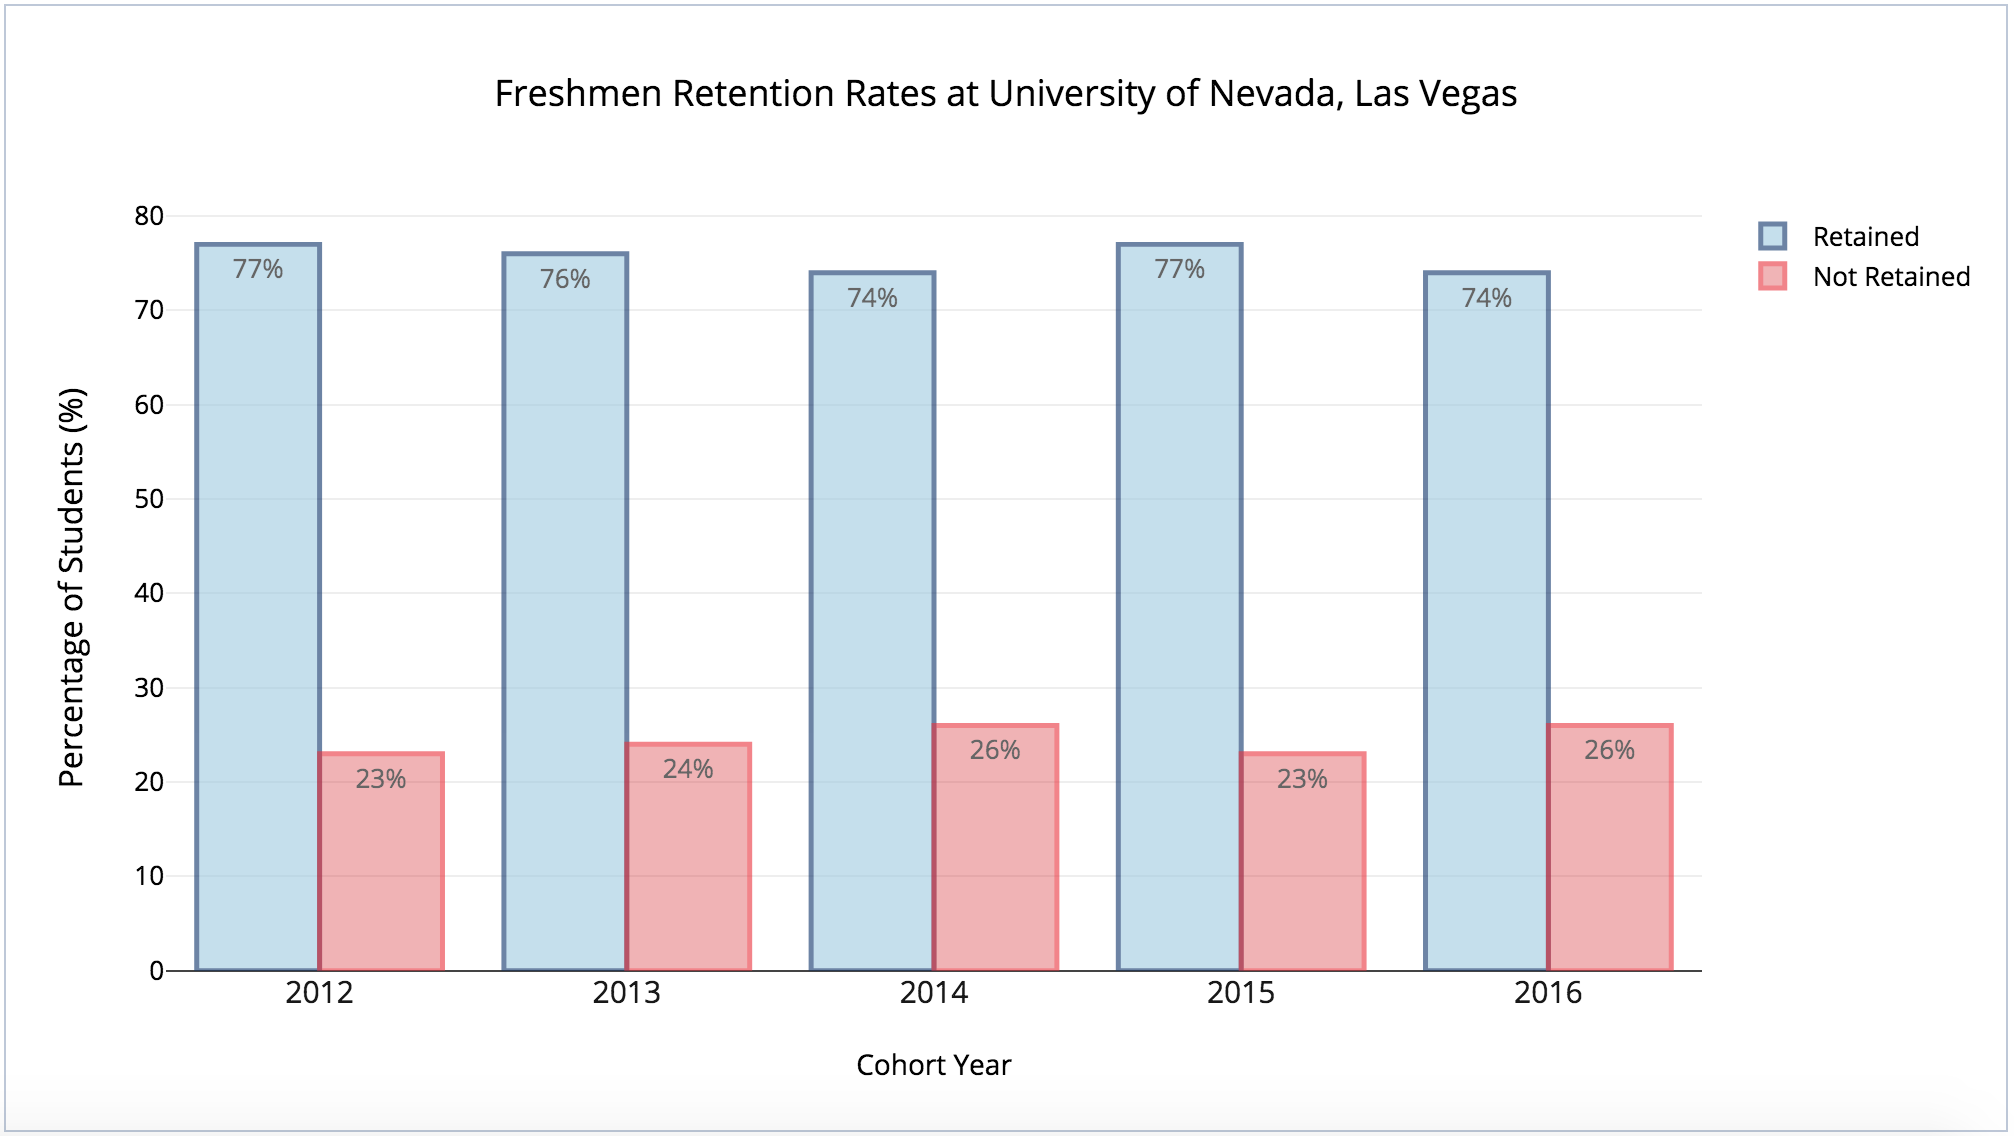
\includegraphics[scale=0.5]{freshmen_rates}
	\caption{Freshmen Retention Rates at UNLV}
	\label{fig:unlv_retention_trend}
\end{figure}

\section{Objective}\label{section:objective}
The objective of this thesis is to create predictive models that can be used to identify at-risk students. In this thesis, important machine learning algorithms such as Logistic Regression, Decision trees, Random Tree Classifiers and SVM's will be trained on real-time student data obtained from UNLV's enrollment census. The trained models will then be used to predict at-risk students from a test dataset which the model has not seen earlier. The models are evaluated and compared using metrics such as precision, recall, and area under the curve to determine which model provides the best results. The results of the analysis such as the evaluation metrics will be converted to risk scores which can be easily understood by the educators and administrators at UNLV. Another contribution of this thesis is to rank students based on risk scores which will be very helpful in an efficient allocation of resources as part of the intervention programs.

\section{Outline}\label{section:outline}

In Chapter \ref{chapter:introduction}, the brief topic of First-Year student retention rates, its importance to universities and the proposed approach to increase the retention rates at UNLV was described.\newline

\noindent In Chapter \ref{chapter:background}, we will discuss the existing research on improving first-year retention rates and the background information required to understand the proposed predictive approach using machine learning. It will also cover the most important and popular algorithms of machine learning.
\newline

\noindent In Chapter \ref{chapter:methodology}, we will describe the methodology adapted for the analysis. The characteristics of datasets used for these methods will also be described.
\newline

\noindent In Chapter \ref{chapter:building_models}, we will present the experimental results. The characteristics of datasets used for these methods will also be described.
\newline

\noindent In Chapter \ref{chapter:conclusion}, we will summarize the proposed methods and their results along with the possible extension of this thesis.

\chapter{Background and Preliminaries} \label{chapter:background}
\section{Related Work}\label{section:relatedwork}

The prediction of first-year student retention rates and identification of students at risk of not being retained has been a well-researched problem in the area of higher education sector for decades. Early studies involved learning the important factors that lead to student dropout by developing a theoretical model. Tinto is one of the major and earliest researchers in this area. Tinto's student engagement model \cite{tinto1999taking} has served as the basis for a large number of theoretical studies \cite{braxton2002introduction}. Similar research was carried out by Ernest Pascarella, Patrick Terenzini, and Alexander Astin, which focused more on the external factors such as the institution's administration and its policies when determining the reasons for student retention \cite{astin2012assessment}. Tinto in his 2006 study \cite{tinto2006} has stated that there has been a huge increase in the number of businesses and organizations to analyze and help institutions with the student retention problem. Later, in the same study, he revealed that there was only little change in the retention rates even with some huge businesses helping the universities. He also described the importance of external factors such as student-faculty relationships, extracurricular program, and orientation programs for first years. Moreover, he incorporated the role of academic factors into his model to make it more suitable to the college structure \cite{tinto2006}. Astin in his Input-Environment model \cite{astin2012assessment}, suggests that researchers should consider pre-college factors such as gender, race/ethnicity, family background, high school GPA  as important for student retention.

In addition to understanding the factors responsible for student dropout, the researchers were interested in identifying students at risk of not being retained in order to intervene and prevent them from dropping out. Early research included usage of statistical and analytical methods such as logistic regression and discriminant analysis for predicting student retention rates \cite{lakkaraju2015machine,marbouti2016models,adejo2017}. The results from these models showed that the learning algorithms were in fact better than many existing rule based models in learning patterns from the existing student data. Educational data mining has emerged into an important field of research in studying student retention, because of its high accuracy and robustness in working with missing data \cite{alkhasawneh2014developing}. In another study, Jay Bainbridge, James Melitski, Anne Zahradnik, Eitel J. M. Lauría, Sandeep Jayaprakash and Josh Baron used fall 2010 undergraduate students data from four different sources and applied classifiers such as logistic regression, support vector machines and c4.5 decision trees for prediction and comparison purposes\cite{bainbridge2015}. The results showed that logistic regression and SVM trees provided higher classification accuracies compared to the decision trees to predict students at risk. 

Serge Herzog a researcher from University of Nevada, Reno(UNR) campus has done some extensive research on student retention and graduate prediction. He used Decision trees and Neural networks to predict student retention of data from UNR\cite{herzog2006estimating}. FarshidMarbouti, Heidi A.Diefes-Dux, KrishnaMadhavan \cite{marbouti2016models} have compared seven different prediction models for identifying at-risk students using in-semester performance factors (i.e., grades) and based on standards-based grading.Another similar research focused on the problem of imbalanced output class distribution in the field of student retention in which the researchers tested three balancing techniques such as over-sampling, under-sampling and synthetic minority over-sampling (SMOTE) along with machine learning algorithms \cite{thammasiri2014critical}.

Although predictive analysis using machine learning models have proved to be very effective in identifying at-risk students, they were still not efficient and useful to educators who wanted to develop academic support programs and resources to support the identified students. The primary reason being the lack of understanding of the metrics from the predictive models by the educators. A few researchers analyzed this issue at the high school level and came up with a framework to convert model accuracies to risk scores that could be used by the educators in the efficient allocation of the resources \cite{lakkaraju2015machine}. Though the above-mentioned framework was giving good results, it was restricted to school level data and thus cannot yield accurate results in the university level as both are very different environments with different set of factors. Hence, in this thesis we try to include such an analysis into college level studies of UNLV and compare our results to the existing approaches.


\section{Preliminaries}\label{section:preliminaries}

\subsection{Machine Learning Concepts}

\noindent  Tom Mitchell defined Machine Learning as \cite{Mitchell1997}: 
\newline\newline
\hangindent=0.7cm "A computer is said to learn from experience E with respect to some class of tasks T and performance measure P, if its performance at tasks in T, as measured by P, improves with experience E." \newline 

\noindent Example: playing chess.

\noindent E = the experience of playing many games of chess with different people

\noindent T = the task of playing chess.

\noindent P = the probability that the program will win the next game.\newline 

\noindent In general, machine learning tries to learn patterns inherent in the underlying data and remembers it as experience, which it uses for predictions. It was conceptualized from the notion of learning process adopted by a human brain. Just as the human brain gets better at a specific task by repeated learning and previous experiences, a computer will also learn more patterns hidden in the data based on its previous experiences. Additionally the huge processing power of computers enables them to perform such a learning process in identifying patterns from complex data which can be very difficult for a human to understand. 

\subsection{Predictive Analytics}
Predictive analytics primarily deals with extracting patterns using machine learning models from existing datasets. the extracted patterns are used to predict future events and behaviors in previously unseen data. Predictive analytics is being used in wide range of fields such as education, finance, automobile, and healthcare. The analytics is performed by running different machine learning algorithms on previously collected data. The algorithms try to learn patterns between different properties of the data and preserve the knowledge in model parameters. The resulting model is able to predict the unknown property of a future unseen data. 

 \begin{table}[!t]
	\renewcommand{\arraystretch}{1.3}
	\caption{Admissions data at a University}
	\label{table:example_db}
	\centering
	\begin{tabular}{|c|c|c|c|c|}
		\hline
		\bfseries Age & \bfseries Gender & \bfseries HSGPA & \bfseries ACT & \bfseries Accepted\\
		\hline
		$20$ & Male & 3.89 & 25.6 & 1\\ \hline
		$21$ & Female & 3.20 & 22.6 & 1\\ \hline
		$20$ & Female & 2.50 & 18.3 & 0\\ \hline
		$22$ & Male & 3.10 &  19.2 & 0\\ \hline
		$19$ & Female & 3.60 & 23.5 & 1\\ \hline
	\end{tabular}
\end{table}


An illustrative example is shown in Table \ref{table:example_db} which shows student data captured during admissions at a university. The aim is to predict if the student will be accepted or not by looking at the other variables in the data. The column "Accepted" is said to be a dependent variable, and all the other variables are called independent variables. A "1" in the "Accepted" column represents the outcome of the student being accepted into the university and a "0" means he was rejected. To this data we apply a machine learning algorithm, that will learn a prediction model based on the relations between the input independent variables and the output dependent variable. The learned model is then able to predict the output variable by taking other variables as input. The output variable can be of any data type. If it is a continuous numerical value, then the machine learning problem is known as regression and if it is categorical value, then the machine learning problem is known as classification.
  \begin{figure}
	\centering
	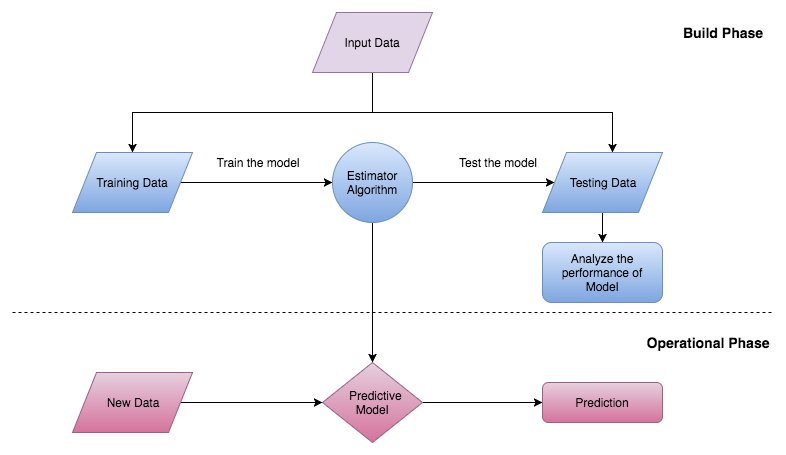
\includegraphics[scale=0.5]{MLApproachFinal}
	\caption{Machine Learning Approach}
	\label{fig:predictive_analysis-approach}
\end{figure} 

The general approach for applying predictive analysis on a data can be divided into 2 phases as shown in figure \ref{fig:predictive_analysis-approach}. Build phase deals with the process of creating a prediction model and testing its performance. The process of creating the prediction model is known as training and the data used is known as training data. To test the effectiveness of the created model, it is tested on another set of previously unseen data known as testing data. We use two different data sets to check the generalization capacity of the model in predicting previously unseen data. If we use all the available data for training, the model may learn too much from the inputs giving rise to the problem of overfitting. Overfitting occurs when a model is performing well on its training data, but not on the other unseen data. A common approach to handle the problem of overfitting is to divide the input data into training and testing sets. The model is then evaluated for performance using test data.  The evaluated model is used in the operational phase to perform predictions given a new data. The metrics used to evaluate a model are explained in detail in coming chapters.


\subsection{Selected Models}
Based on the way machine learning algorithms "learn" patterns from data, they can be classified into two groups: supervised and unsupervised learning. In supervised learning, we train the machine learning model using data whose possible outcomes are already known, whereas unsupervised learning is the training of machine learning models using information that is neither classified nor labeled and allowing the algorithm to learn by itself. 

In our case, since we have data about students along with the labels of the outcome variable, we will do supervised learning. Additionally, the outcome variable in our analysis is a categorial variable, indicating if the student was retained in their second year or not and thus our problem is of classification. In this section we discuss various classification models that were used in this thesis to analyze the student data from UNLV. The models selected for comparison were Logistic Regression, Decision Trees, Random Forest, and SVM's.

\subsubsection {Logistic Regression Model}

Logistic Regression is a supervised machine learning classification algorithm that is used to predict the probability of a categorical dependent variable. In logistic regression, the dependent variable is a binary variable that contains data coded as 1 (yes, success, etc.) or 0 (no, failure, etc.). It is a variation of linear regression, where a model is constructed in supervision of the available data to calculate the unknown outcome variable. In linear regression, input values (x) are combined linearly using weights or coefficient values to predict an output value (y), whereas logistic regression calculates the probability of getting the outcome dependent variable (y). The general equation for this learning approach with one independent variable and a dependent output variable 'y' is as shown in the Equation\ref{eq:logistic} 
\begin{equation}
 P(y=1)= g(\beta0+\beta1 *x )  \label{eq:logistic} 
 \end{equation}
 where the coefficient '$\beta$0' is the bias and \lq$\beta$1\rq  is the coefficient for the single input value (x) which are learned from the available input data during training and 'g' is a mathematical function known as Sigmoid function, that maps the linear combination of inputs into the range of [0,1], thus giving us probabilities and is defined as shown in the Equation\ref{eq:sigmoid}. For the case of multiple independent input variables, the input values (x) are represented as a vector X along with equal number of coefficients to be learned.
 
\begin{equation}
 g(z) =  \frac{\mathrm{1} }{\mathrm{1} + e^- z }  \label{eq:sigmoid} 
 \end{equation}

As an illustrative example, consider the problem of identifying if a student will pass an exam based on the number of hours he studies before the exam. In this case, we can define the input independent variable as the number\_of\_hours\_studied which takes a numerical value and the output variable as Student\_Passed which takes values { 0 or 1 }. Hence our logistic regression problem then represents the probability of the student passing an exam given the number of hours he studied before the exam. A rule of thumb in logistic regression is if the probability is $>$ 0.5 then the decision is true. Hence you end up with a model that finds the probability of a student passing the exam  as shown in Equation\ref{eq:logisticExample}

\begin{equation}
 P(y=1) = P(Student\_Passed= True) = 0.82 * (number\_of\_hours\_studied) -0.32.  \label{eq:logisticExample} 
 \end{equation}


\subsubsection {Decision Trees}

A decision tree is a supervised machine learning algorithm which is mostly useful for classification problems and works for both continuous and categorical input and output variables. In simple terms, a decision tree uses the tree representation to solve the problem, in which each branch represents a choice between a number of alternatives of an attribute in the internal nodes leading to a final decision in the leaf node. Decision trees where the output variable is categorical are known as Classification trees.

  \begin{figure}
	\centering
	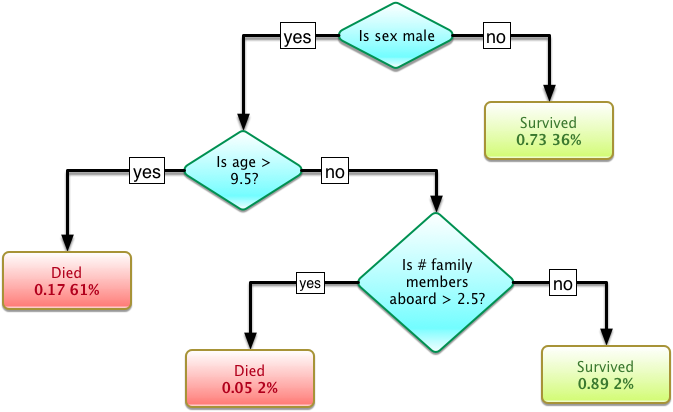
\includegraphics[scale=0.5]{titanic-decision}
	\caption{Classification tree of passenger survival in Titanic}
	\label{fig:classification_tree_titanic}
\end{figure} 

The general approach of constructing a decision tree from the training data involves splitting the entire data at the root node into a subset based on a requirement (generally, a decision on an attribute). The process of splitting based on decisions of different internal node attributes continues until a subset at a node has all the same value of the target variable, or when splitting no longer adds value to the predictions. The main goal of decision trees is to find the best split of each node of the tree. But measuring the "goodness" of a given split is a subjective question so, in practice, different metrics are used for evaluating splits. Two main metrics used to evaluate the splits are :
\begin{description}
    \item[Gini impurity] : It is a measure of how often a randomly chosen element from the set would be incorrectly labeled if it was randomly labeled according to the distribution of labels in the subset. It reaches its minimum (zero) when all cases in the node fall into a single target category. 

    \item[Information gain] : For each node of the tree, the information gain value represents the expected amount of information that would be needed to specify whether a new instance should be classified yes or no, given that the example reached that node. The node with highest information gain value yields the best split. 
     
 \end{description}
 
For illustration purpose, consider the classification tree showing survival of passengers on the Titanic ship when it sinked in Figure \ref{fig:classification_tree_titanic}. The figures under the leaf nodes show the probability of survival and the percentage of observations in the leaf. The tree was constructed using gini impurity as the goodness evaluation metric. From the tree we can make the following inferences: 
\begin{enumerate}
  \item If the passenger is a male and has an age greater than 9.5 then he did not survive the titanic sink.
  \item All the female passengers had a survival probability of 0.73.
  \item If the passenger was male, had an age less than 9.5 and had lesser than 2.5 family members aboard survived the sink with a probability of 0.89.
\end{enumerate}


\subsubsection {Random Forest Classifiers}
Random forest classifier is another supervised machine learning algorithm that can be used for both classification and regression problems. It is generally classified into a special type of machine learning method known as an Ensemble method in which a combination of weak classifiers is used to form a strong classifier which can be used to perform better predictive analysis. In case of the random forests, decision trees are the weak learners.  Although decision trees perform really well on some datasets, they are generally called weak learners as they tend to have high variance when they are trained on different subsections of the same data. Here, variance refers to the spread of the predictions and occurs when a model is sensitive to small changes in the training data which is the case of overfitting. This happens due to the greedy approach employed by decision tree algorithm along with information gain or gini index metrics, to learn rules from the training data.
  \begin{figure}
	\centering
	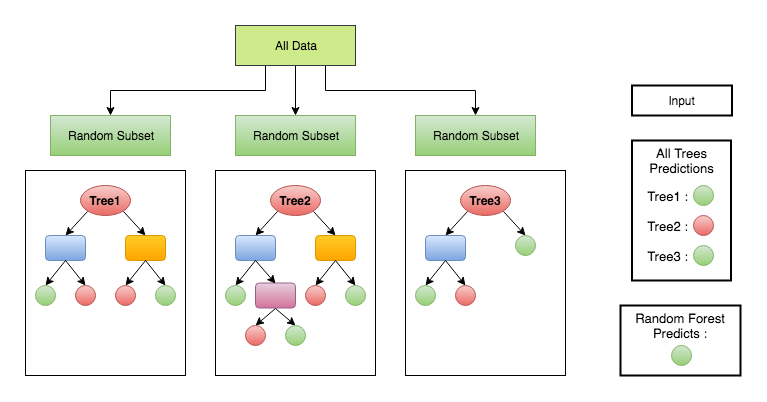
\includegraphics[scale=0.6]{randomforests}
	\caption{Random forest trees}
	\label{fig:random_forest_trees}
\end{figure} 


Random forests on the other hand create a number of decision trees during training by using different subsections of the training data.  Moreover the process of finding the root node and splitting the feature nodes occurs randomly in random forests. Once we have a forest of trees, decisions from different trees are combined to make a final decision regarding the data. This way the random forests will generalize the predictions better as the combination of decisions will not be sensitive to the trained data as each tree learns from different subsections of data. The more the number of trees in the random forest the better generalized are the predictions.


The figure \ref{fig:random_forest_trees} explains the construction of random forests from the available input data. The initial training data is split into random subsets using which individual decision trees are constructed. The trees constructed from different subsets can have a different structure. Once we have the random forest, when a new input is given, it makes a prediction by using a voting of results from all the trees as shown in the figure.

\subsubsection {Support Vector Machines }

Support Vector Machine (SVM) is a supervised machine learning algorithm which can be used for both classification and regression problems. It is commonly known as a large margin classifier and is mostly useful for classification problems. In this algorithm, each data item with n features is plotted as a point in an n-dimensional space with the value of each feature being the value of a particular coordinate. Then, classification is done by finding the hyper-plane that separates the two classes very well. A hyperplane is a line that splits the input variable space.

As an example, consider a binary classification problem with one input variable (x) and one output variable (y), which can be easily visualized in a two-dimensional space as shown in Figure \ref{fig:svm_example}. The SVM classifier tries to find a hyperplane that separates all of the input points (in this case a line). After the line that separates the input data well is obtained, it can be used to make classifications by plugging in input values. If the equation returns a positive value, then the point is classified as being in the first class and if its a negative value, then the point is classified as being in the second class. Alternatively, a point close to the line returns a value close to zero and it may be difficult to classify it. The perpendicular distance between the line and the closest data points is referred to as the margin. The best line that can separate the two classes is the line that has the largest margin. Thus the name Large-Margin classifier. These closest points play an important role in defining the line and in the construction of the classifier and thus are called the support vectors. The hyperplane is learned from the training data using an optimization procedure that maximizes the margin.

  \begin{figure}
	\centering
	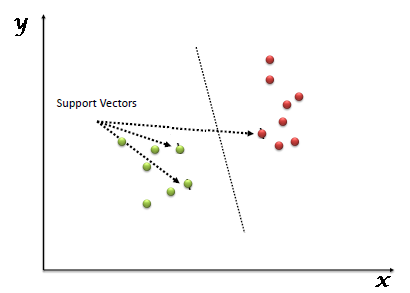
\includegraphics[scale=0.6]{svm_example}
	\caption{Example SVM Classifier}
	\label{fig:svm_example}
\end{figure} 

In practice, real world data is messy and cannot be perfectly separated with a hyperplane. In such cases, the SVM tries to relax the constraint of maximum margin hyperplane by allowing some points in the training data to violate the separating hyperplane principle. This is generally done by varying a tuning parameter known as 'C' which defines the amount of the violation allowed by the classifier. The general approach is to try different values of C and chose the one that is best for the data.

In SVM, it is easy to have a linear hyper-plane between the two classes. However, to create hyperplanes that separate non-linear data, SVM uses a technique called the kernel trick. In the kernel trick, SVM uses functions which takes the low dimensional non separable input space and transforms it into a higher dimensional separable space. The functions used are known as kernels. The most commonly used kernels are linear kernels, polynomial kernels and radial kernels. 

\subsection {Evaluation Methods}
In this subsection, we will explain the various evaluation methods that are used in this thesis to assess and compare the performance of different models.

In machine learning, the problem at hand is of making good predictions on unknown and unseen data by the learned models. In simple terms, we want to know for sure how well the model is able to generalize new unseen data and ensure that it is not just memorizing patterns in the data. To make a better analysis of the generalizing power of the model, the data is generally split into training and testing sets, where training data is used to create the model while testing set to evaluate the model. To do this, we need to define the performance measure strategies we will use to evaluate our models. Having a performance measure defined for the machine learning problem also gives us the advantage of focusing our time effectively on improving our model predictions. We generally use the term 'metric' to refer to a performance measure in machine learning. Various metrics are available depending on whether the problem is of  classification or regression. Since we are dealing with a classification problem in this thesis, we will concentrate more on the metrics for a classification problem.

\subsubsection {Confusion Matrix}
Confusion matrix is a representation of the predictions made by the classification model. It is a very important and useful metric in classification problems as it can not only be used to represent the models performance by itself but can also compute other metrics. A confusion matrix is composed of statistics such as true positives, true negatives, false positives, and false negatives, which are calculated using actual and predicted values. The idea of such a representation was to understand how many times the model was right in predicting a true or false value and how many times it failed to do so.

  \begin{figure}[!htbp]
	\centering
	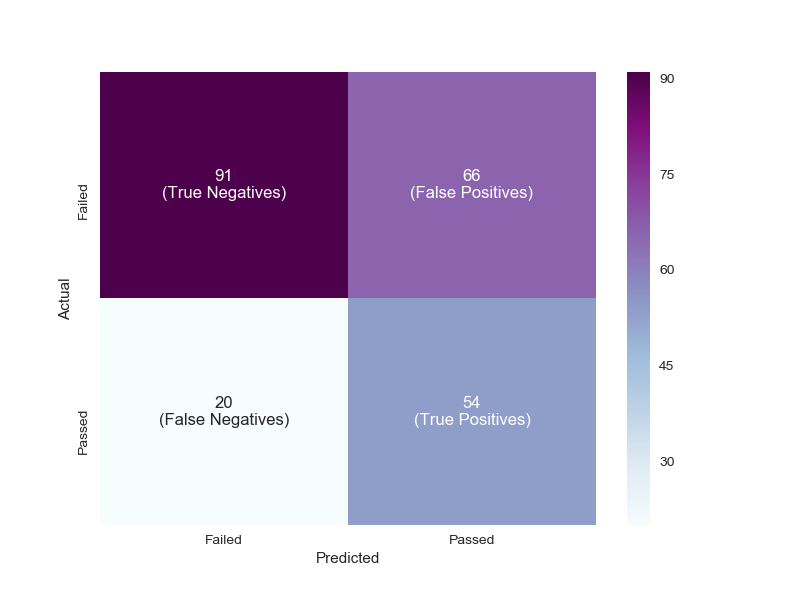
\includegraphics[scale=0.6]{Confusion_matrix}
	\caption{Example Confusion Matrix}
	\label{fig:example_confusion_matrix}
\end{figure} 

To help understand the concepts of the confusion matrix representation, an example confusion matrix is shown in Figure \ref{fig:example_confusion_matrix}. The matrix was generated from a total population of 231 students, where the predictions represent if the student passed a certain exam or not. 
\begin{description}
    \item[True Positive] : The case where the actual value was true and the model also predicted it as true is known as a True Positive. The total number of such true positives from the population are represented on the top left corner of the confusion matrix. In Figure \ref{fig:example_confusion_matrix}, the total number of true positives is 54 out of the total population of 231.

    \item[False Negative] : The case where the actual value was true and the model predicted it as false is known as a False Negative. The total number of such false negatives from the population are represented on the top right corner of the confusion matrix. In Figure \ref{fig:example_confusion_matrix}, the total number of false negatives is 20 out of the total population of 231.

     \item[False Positive] : The case where the actual value was false and the model predicted it as true is known as a False Positive. The total number of such false positives from the population are represented on the bottom left corner of the confusion matrix. In Figure \ref{fig:example_confusion_matrix}, the total number of false positives is 66 out of the total population of 231.
     
      \item[True Negative] : The case where the actual value was false and the model also predicted it as false is known as a True Negative. The total number of such true negatives from the population are represented on the bottom right corner of the confusion matrix. In Figure \ref{fig:example_confusion_matrix}, the total number of true negatives is 91 out of the total population of 231.
     
 \end{description}
 The confusion matrix in Figure \ref{fig:example_confusion_matrix} is for a binary classification problem with 2 classes \{'Passed', and 'Failed'\}. For a multi-class classification problem, each class has a row and a column in the confusion matrix and the problem is generally analyzed as a one-vs-all problem.


\subsubsection{Classification Accuracy}
Classification accuracy is the proportion of number of correct predictions to all the predictions made by the model. This is the most common evaluation metric for classification problems. It can be calculated by using the values in the confusion matrix as the ratio of the sum of true positives and true negatives to the total size of the predicted population. The Equation \ref{eq:classificationAccuracy}  represents the calculation of classification accuracy.

\begin{equation}
Classification\, Accuracy = \dfrac{True\, Positives + True\, Negatives}{size\, of\, predicted\, population} \label{eq:classificationAccuracy} 
 \end{equation}

The classification accuracy calculated from the confusion matrix shown in Figure \ref{fig:example_confusion_matrix} would be (54+91)/231, which is 0.63.

\subsubsection{Sensitivity}

Sensitivity describes the probability of the prediction being true when the actual class is true. In simple terms, it describes how sensitive the model is when predicting positive instances. It is also known as "True Positive Rate" or "Recall" and is calculated as the ratio of true positives to the actual true cases. It can be calculated by using the values in the confusion matrix as the ratio of true positives to the sum of true positives and false negatives. The Equation \ref{eq:Sensitivity}  represents the calculation of sensitivity.

\begin{equation}
Sensitivity = \dfrac{True\, Positives }{True\, Positives\, + False\, Negatives} \label{eq:Sensitivity} 
 \end{equation}

The sensitivity calculated from the confusion matrix shown in Figure \ref{fig:example_confusion_matrix} would be 54/(54+20), which is 0.73.


\subsubsection{Specificity}

Specificity describes the probability of the prediction being false when the actual class is false. In simple terms, it describes how specific the model is when predicting negative instances. It is calculated as the ratio of true negatives to the actual false cases. It can be calculated by using the values in the confusion matrix as the ratio of true negatives to the sum of true negatives and false positives. The Equation \ref{eq:Specificity}  represents the calculation of specificity.

\begin{equation}
Specificity = \dfrac{True\, Negatives }{True\, Negatives\, + False\, Positives} \label{eq:Specificity} 
 \end{equation}

The specificity calculated from the confusion matrix shown in Figure \ref{fig:example_confusion_matrix} would be 91/(91+66), which is 0.58.

\subsubsection{Precision}
Precision defines the probability of the prediction being correct when the model identified it as true. In simple terms, it describes how precise the model is when predicting positive instances. It is calculated as the ratio of true positives to the predicted true cases. It can be calculated by using the values in the confusion matrix as the ratio of true positives to the sum of true positives and false positives. The Equation \ref{eq:Precision}  represents the calculation of precision.

\begin{equation}
Precision = \dfrac{True\, Positives }{True\, Positives\, + False\, Positives} \label{eq:Precision} 
 \end{equation}

The precision calculated from the confusion matrix shown in Figure \ref{fig:example_confusion_matrix} would be 54/(54+66), which is 0.45.

\subsubsection{F\textsubscript1 Score}

F\textsubscript{1} score is calculated by taking a harmonic mean of the precision and recall of the model's predictions. It is also known as F-measure or balanced F-score. The Equation \ref{eq:Precision}  represents the calculation of precision.

\begin{equation}
F_{1} = \dfrac{True\, Positives }{True\, Positives\, + False\, Positives} \label{eq:Precision} 
 \end{equation}

The F\textsubscript{1} score calculated from the confusion matrix shown in Figure \ref{fig:example_confusion_matrix} would be 0.56.


\subsubsection{Area Under Curve (AUC)}

In binary classification problems, the general rule of thumb is to use a probability threshold of 0.5 to make classification predictions. But for few scenarios, this threshold might not hold good and using a different threshold would be more appropriate. An Receiver Operating Curve (ROC) is the most commonly used way to visualize the performance of a binary classifier for different thresholds. It is obtained by plotting the True Positive Rate against the False Positive Rate. False positive rate is calculated as (1 - Specificity). From the ROC plot, we can calculate the Area under the curve (often referred to as simply the AUC) which is the probability that a classifier will rank a randomly chosen positive instance higher than a randomly chosen negative one \cite{fawcett2006introduction}.


  \begin{figure}[!htbp]
	\centering
	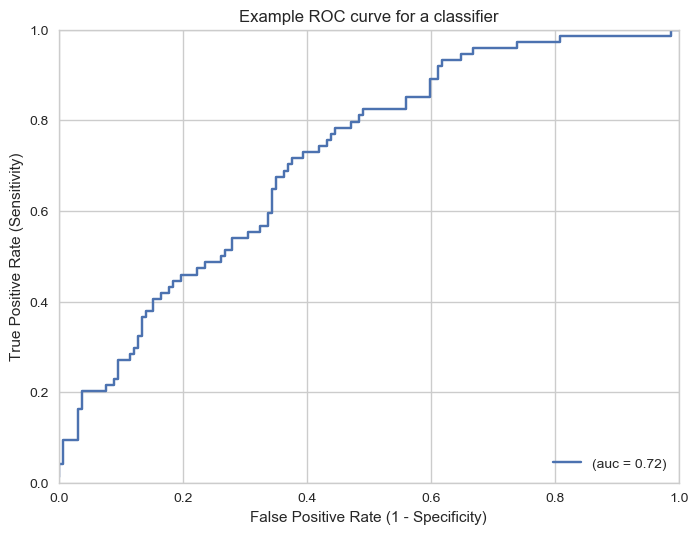
\includegraphics[scale=0.6]{ExampleROC}
	\caption{Example ROC curve}
	\label{fig:example_roc}
\end{figure} 

The Figure \ref{fig:example_roc} shows the roc curve constructed from our example data captured by confusion matrix in the Figure \ref{fig:example_confusion_matrix}. In the plot, the area under the blue line refers to the AUC of the classifier, which in this case is (0.72). The dashed line in the diagonal represents the ROC curve of a random predictor.

\subsubsection{Cross Validation}
So far, we discussed the calculation of various metrics based on the predictions obtained from a single test data which was split from the original data. The approach of dividing the input data into training and testing data is known as holdout method. The typical split rate is about 70\% of input data into training and remaining 30\% into testing data. These splits are generally created by random sampling. One problem with the holdout strategy to evaluate the models performance is that the random splits might not be fair and lets say a specific combination of input data might always end up in testing data about which the model will have little information since it did not see them during training. As a result the model cannot make good predictions on them. To tackle with such scenarios, we use a method known as Cross Validation. 

In Cross validation, the machine learning models are trained on several subsets of the available input data and evaluated on the complementary subset of the data. There are several available strategies based on the way the subsets are split. K-Fold cross validation and Stratified K-Fold cross validation are among the most popular and frequently used strategies.

In K-Fold cross validation, the data is divided into k subsets. In simple terms, the holdout method is repeated k times, such that each time, one of the k subsets is used as the test set/ validation set and the other k-1 subsets are put together to form a training set. The error estimation is averaged over all k trials to get total effectiveness of our model. As can be seen, every data point gets to be in a validation set exactly once, and gets to be in a training set k-1 times. This significantly reduces bias as we are using most of the data for fitting, and also significantly reduces variance as most of the data is also being used in validation set. Interchanging the training and test sets also adds to the effectiveness of this method. The typical value of K suggested by many researchers is 10.

Stratified K-Fold cross validation is actually a variation of the K-fold cross validation which works better when applied on data that has huge imbalance in the response variable. In this approach, each fold contains approximately the same percentage of samples of each target class as the complete set.\newline

\noindent In this subsection, we discussed about classification accuracy, sensitivity, specificity, recall, AUC and cross validation. Among the evaluation metrics, sometimes the classification accuracy can be a bad indicator of the model performance as it requires the output classes distribution in the original set to be balanced which is rarely true for real world datasets. As for other metrics, it becomes hard to compare three to four values to identify the model that performs best. Hence, in these cases F\textsubscript1 score and AUC can be used as a single value comparators of the models performances. Moreover, applying cross validation strategies to calculate the metrics would give evaluation measures that describe the model performance with higher confidence.



\chapter{Methodology} \label{chapter:methodology}
\section{Data Collection}

The Operations Support and Reporting Office at UNLV is responsible for extracting information regarding student enrollment and performance from the UNLV Data Warehouse and reporting the census to Integrated Postsecondary Education Data System (IPEDS). The data used in this thesis were obtained from the census data submitted to IPEDS every year. The following subsections will describe more information about the data.

\section {Data Preparation}
\subsection{Data Description}
The census data from the Operations Support and Reporting Office was exported into a csv file to be used by the analysis. The raw data consisted of a total of 17,708 freshmen student records captured cohort-wise from the academic year 2012 to 2016. The data consisted of a variety of information about each student, such as pre-college academics, standardized test scores, the social and economic status of the student, freshmen year academics and finally if the student was retained in the sophomore year. On the whole, a total of 41 attributes were captured for each student. Table \ref{table:long_data_description_db} describes the variables and their types. The following subsections describe in detail about the dataset. 

 \begin{longtable}{|c|l|l|l|}

\caption{Description of data fields for first-year student data}\\
\hline
\textbf{No.} & \textbf{Feature} & \textbf{Type} & \textbf{Description} \\
\hline
\endfirsthead
\multicolumn{4}{c}%
{\tablename\ \thetable\ -- \textit{Continued from previous page}} \\
\hline
\textbf{No.} & \textbf{Feature} & \textbf{Type} & \textbf{Description} \\
\hline
\endhead
\hline \multicolumn{4}{r}{\textit{Continued on next page}} \\
\endfoot
\hline
\endlastfoot
\label{table:long_data_description_db}
		1 	& Cohort\_Year 		&	Multi Nominal 	&	 First Fall Academic year of the student\\ \hline   
		2 	& SummerAdmit 		& 	Binary Nominal 	& 	If Student was admitted in prior summer \\ \hline
		3 	& AltAdmit 			& 	Binary Nominal	& 	If Student was Transferred or admitted differently \\ \hline
		4 	& F1\_EnrollCredits		&	Numerical		&	Count of semester credits enrolled for admit term \\ \hline
		5	&F1\_MidtermGPA		&	Numerical		&	F1 mid-term GPA \\ \hline
		6 	& F1\_GPA 			&	Numerical		&	Term GPA for first fall term (admit term) 	\\ \hline
		7	&F1\_Math\_Type		&	Multi Nominal	&	Type of Math Course Taken in F1 term \\ \hline
		8	&F1\_MathGradePass	&	Binary Nominal &	F1 Math Grade Passed or Failed		\\ \hline
		9 	&F1\_GPA\_units		&	Numerical		&	Units completed in first fall (for GPA)		\\ \hline
		10 	&F1\_Complete		&	Binary	Nominal	&	Completed first fall term (final census)		\\ \hline
		11 	&S1\_Retain			&	Binary	Nominal	&	Enrolled in 1st spring (S1) - yes or no			\\ \hline
		12 	&S1\_EnrollCredits		&	Numerical		&	Count of semester credits enrolled for S1 term \\ \hline
		13	&S1\_GPA\_units		&	Numerical		&	Units completed in S1 (for GPA)			  \\ \hline
		14	&S1\_MathTaken		&	Binary Nominal &	If Math taken in S1 term 			\\ \hline
		15	&S1\_GPA			&	Numerical		&	Term GPA for S1 term				\\ \hline
		16 	&S1\_Complete		&	Binary	Nominal	&	If student completed S1 term			\\ \hline
		17	&Yr1\_MathTakenOverall & Multi Nominal		&	Type of Math taken in First year			\\ \hline
		18 	&Mom\_Edu\_Level		&	Multi Nominal		&	Highest education level of Mother		\\ \hline
		19 	&Dad\_Edu\_Level		&	Multi Nominal		&	Highest education level of Father			\\ \hline
		20 	&First\_Gen			&	Binary Nominal	&	If the kid is the first to attend college		\\ \hline
		21 	&Gender			&	Binary Nominal	&	Student Gender					\\ \hline
		22 	&Housing			&	Multi Nominal		&	on or off-campus housing				\\ \hline
		23 	&IPEDS\_Race		&	Multi Nominal		&	IPEDS race/ethnicity data				\\ \hline
		24 	&Marital\_Status		&	Multi Nominal		&	Marital status of the student in admit term	\\ \hline
		25 	&CoreHSGPA			&	Multi Nominal		&	Core high school GPA of the student		\\ \hline
		26 	&UnwHSGPA			&	Multi Nominal		&	Unweighted high school GPA of the student	\\ \hline
		27 	&SAT\_ACT\_Score		&	Numerical		&	ACT scores scaled to SAT scores			\\ \hline
		28 	&ACT\_SAT			&	Binary Nominal	&	If the student has taken ACT or SAT		\\ \hline
		29 	&F1\_Residency		&	Binary Nominal	&	In state or Out of State in F1 term		\\ \hline
		30 	&F1\_TuitionRes		&	Multi Nominal		&	Tuition status of the student in F1 term \\ \hline
		31	&F1\_MillScholar		&	Binary Nominal		& 	1st fall Millennium Scholarship recipient  \\ \hline
		32	&WUE				&	Binary Nominal		&	Western Undergrad Exchange student  \\ \hline
		33	&Age\_Admit\_Pcensus	&	Numerical			&	Age at time of preliminary census of first fall term \\ \hline
		34	&College1				& Multi Nominal			& 	First fall college			\\ \hline
		35	&FA\_INFO\_RECD		&Binary Nominal		&	FAFSA info recorded		\\ \hline
		36	&PELL\_Eligibility		&Binary Nominal		&	If student is eligible for PELL grant \\ \hline
		37	&PELL\_DISB\_AMT &Numerical			&	PELL Grant Disbursed amount \\ \hline
		38	&MILL\_DISB\_AMT		& Numerical			&	Millennium Scholarship disbursed amount	  \\ \hline
		39	&Other\_SCHOL\_AMT & Numerical		&   	Other Scholarships disbursed amount \\ \hline
		40	&LOAN\_DISB\_AMT	&Numerical	&	Student Loan disbursed amount 	\\ \hline
		41	& F2\_Retained			&Binary Nominal &	If the student was retained in Fall 2 term( F2)

\end{longtable}
 
\subsection{Feature Extraction}
Feature extraction involves creating important useful features from the available raw data. Based on the problem statement and the data collection techniques at UNLV. The raw data was used to generate the following important features.

\subsubsection {Computation of SAT\_ACT\_Score Variable}
The admissions office at UNLV requires the students to report scores of standardized exams such as ACT and SAT during their admission process. From the raw dataset, we noticed that the ACT and SAT scores were missing for many students. Especially 56\% of students did not have ACT scores while only 28\% did not have SAT scores. Hence to capture the importance of the standardized scores into our analysis, we converted the available ACT composite scores to equivalent 
SAT composite scores based on the conversion table from \cite{ACTSAT}. The term SAT\_ACT\_Score was used to refer to this converted scores variable.

\subsubsection {Computation of F2\_Not\_Retained Variable}
The main focus of this thesis is to identify the students who are at the risk of not being retained after their freshmen year. In the raw dataset the flag F2\_Retain captures the aspect of student being retained and hence can serve as the outcome variable. We then compute the complement of this flag to obtain the feature F2\_Not\_Retained which takes 0 if the student was retained and 1 if the student was not retained. The problem of identifying students who are at the risk of not being retained after first year is then a binary classification task with F2\_Not\_Retained as the outcome variable.

\section {Data Preprocessing}
Data Preprocessing is a technique that is used to convert the raw data into a clean data set. In other words, whenever the data is gathered from different sources it is collected in raw format which is not feasible for the analysis.
Therefore, certain steps are executed to convert the data into a tiny clean dataset. This technique is performed before the execution of any predictive Analysis. 


\subsection {Handling Outliers in Data}

Generally the process of collecting data from different sources can introduce outliers into the dataset. This may be due to a faulty data extraction program or a human error. In predictive data analysis outliers can have significant effect on the predictive power of the models as they can introduce huge noise into the model. Hence it is almost always essential to check for outliers in the dataset before performing any analysis. Outliers were identified in our dataset. Data plots with index on x-axis and values on y-axis was used to demonstrate the presence of outlier in a feature.


\subsubsection{UnwHSGPA scores}

\begin{figure}
\centering
    \begin{subfigure}[b]{0.55\textwidth}            
            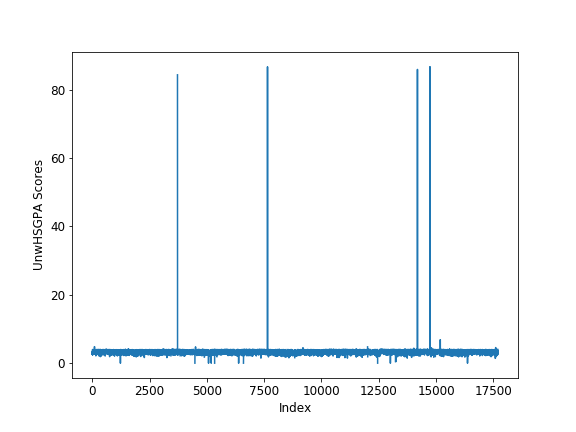
\includegraphics[width=\textwidth]{UnwHSGPAScores}
            \caption{UnwHSGPA with Outliers}
            \label{fig:UnwHSGPA-with-outliers}
    \end{subfigure}%
     %add desired spacing between images, e. g. ~, \quad, \qquad etc.
      %(or a blank line to force the subfigure onto a new line)
    \begin{subfigure}[b]{0.55\textwidth}
            \centering
            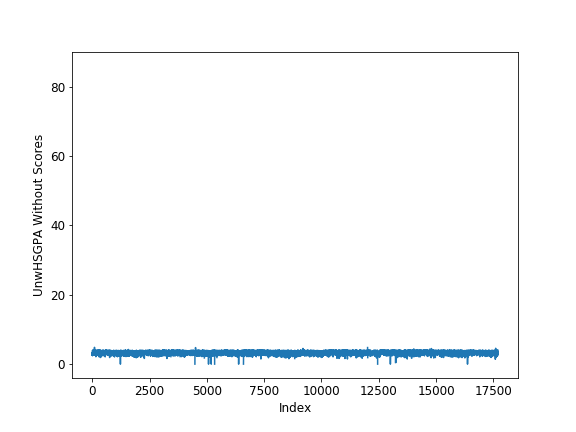
\includegraphics[width=\textwidth]{UnwHSGPAWithoutScores}
            \caption{UnwHSGPA without Outliers}
            \label{fig:UnwHSGPA-No-outliers}
    \end{subfigure}
    \caption{Removing Outliers from UnwHSGPA}\label{fig:unwHSGPA}
\end{figure}

 There were a few outliers identified for variable UnwHSGPA, as shown in figure \ref{fig:UnwHSGPA-with-outliers}. The outliers of the UnwHSGPA were replaced by mean value of the said dataset excluding all the outliers. Data plot of the variable UnwHSGPA after removing outliers is shown in figure \ref{fig:UnwHSGPA-No-outliers}


\subsection {Handling Missing Values}
In this subsection, we will discuss how we handled missing values in the dataset. The table \ref{table:missing_db} shows variables along with the count of missing values. Machine learning deals with the usage of mathematical models on the data and hence it cannot be applied to datasets that have missing values. The general approach is to fill the missing value with a suitable value. The process of filling missing values in the data is known as Imputation. Researchers frequently use the mean, mode or median of the observed given values to substitute in the missing field.
 \begin{table}[!t]
	\renewcommand{\arraystretch}{1.3}
	\caption{Variables with missing values and their count}
	\label{table:missing_db}
	\centering
	\begin{tabular}{|c|c|}
		\hline
		\bfseries Variable & \bfseries Number of missing values \\
		\hline
		SAT\_ACT\_Score & 830\\ \hline
		UnwHSGPA & 1933\\ \hline
		CoreHSGPA & 3463\\ \hline
		F1\_MidtermGPA & 286\\ \hline
		F1\_MathGradePass & 4989\\ \hline
	\end{tabular}
\end{table}

\subsubsection {Imputing SAT\_ACT\_Score}
The SAT\_ACT\_Score variable had 830 missing values. Firstly, to understand the impact of missing values, we calculated the probabilities of the outcomes of  the F2\_Not\_Retained variable with respect to the availability of data points in SAT\_ACT\_Score variable. In one case we ignored the records that had missing values and in other case we included all the records as shown in Table \ref{table:sat_act_db}. By looking at the table, it can be inferred that presence of missing values in SAT\_ACT\_Score variable had very little impact on the percentage of students not being retained. A total of 24.1\% students were not retained when a value was present in the variable and 25.6\% were not retained when the variable had a missing value.

\begin{table}[!t]
	\renewcommand{\arraystretch}{1.3}
	\caption{F2\_Not\_Retained outcome probabilities w.r.t availability of data points  in SAT\_ACT\_Score}
	\label{table:sat_act_db}
	\centering
	\begin{tabular}{|c|l|c|c|}
    \hline
    \multicolumn{2}{|c|}{} & \multicolumn{2}{|c|}{ \bfseries F2\_Not\_Retained }\\ \cline{3-4}
      \multicolumn{2}{|c|}{} & \bfseries 0 & \bfseries 1\\ \hline
     \multirow{2}{*}{ \bfseries SAT\_ACT\_Score}   &  \bfseries Has value & 75.89\% & 24.11\% \\ \cline{2-4}
     & \bfseries Missing value & 74.33\% & 25.67\%\\
    \hline

\end{tabular}
\end{table}


\begin{figure}[!htbp]
	\centering
	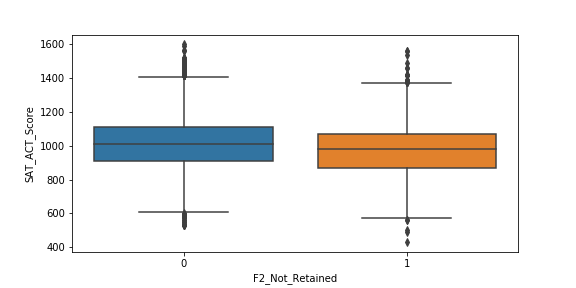
\includegraphics[scale=0.7]{SATBoxPlot}
	\caption{Boxplot of the SAT\_ACT\_Score vs F2\_NotRetained}
	\label{fig:Sat_F2NotRetained_plot}
\end{figure}

Moreover, the boxplot of the SAT\_ACT\_Score vs F2\_NotRetained (Figure \ref{fig:Sat_F2NotRetained_plot}) also shows that SAT\_ACT\_Score has very low impact on the student dropout. Based on the above facts, the missing values in this variable were replaced by the mean value. 

\subsubsection {Imputing CoreHSGPA and UnwHSGPA}
The CoreHSGPA variable had 3463 missing values, whereas the UnwHSGPA had 1943 missing values. Before imputing, we tried to analyze the relation between both the variables (Figure \ref{fig:diffHSGPA}). For this we calculated the difference between CoreHSGPA and UnwHSGPA of available records and plotted them as shown in figure \ref{fig:Core_Unw_diff}. We can clearly observe that majority of the differences were lying in the range of [-1,1], which indicates that the two variables had very close relation. Similar pattern was revealed from the distribution plot of the variable differences as shown in figure( \ref{fig:Core_Unw_dist}), which revealed that the differences followed a gaussian distribution with a mean of 0.23. Based on the above facts, we replaced the missing values with the available variable scores. The remaining missing values were replaced by the mean value of the respective variable.


\begin{figure}[!htbp]
\centering
    \begin{subfigure}[b]{0.55\textwidth}            
            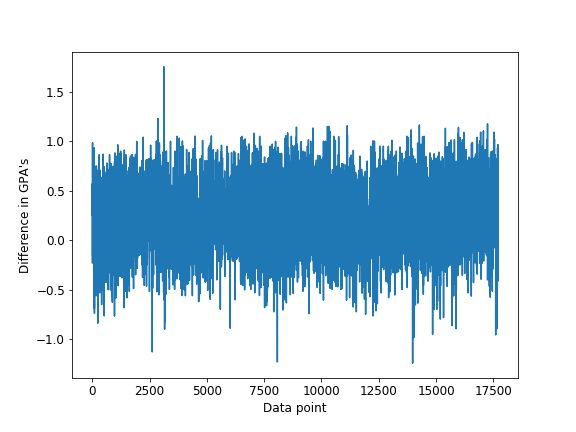
\includegraphics[width=\textwidth]{Core-Unw-GPA-diff}
            \caption{Difference between CoreHSGPA and UnwHSGPA}
            \label{fig:Core_Unw_diff}
    \end{subfigure}%
     %add desired spacing between images, e. g. ~, \quad, \qquad etc.
      %(or a blank line to force the subfigure onto a new line)
    \begin{subfigure}[b]{0.55\textwidth}
            \centering
            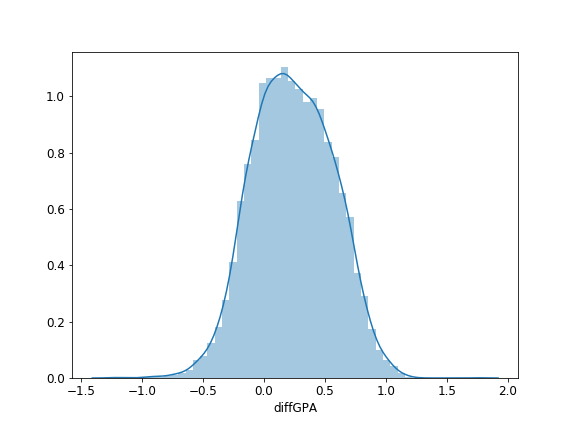
\includegraphics[width=\textwidth]{Core-Unw-GPA-distribution}
            \caption{Distribution }
            \label{fig:Core_Unw_dist}
    \end{subfigure}
    \caption{Analyzing difference between CoreHSGPA and UnwHSGPA }\label{fig:diffHSGPA}
\end{figure}

\subsubsection {Imputing F1\_MidtermGPA}

\begin{figure}[!ht]
	\centering
	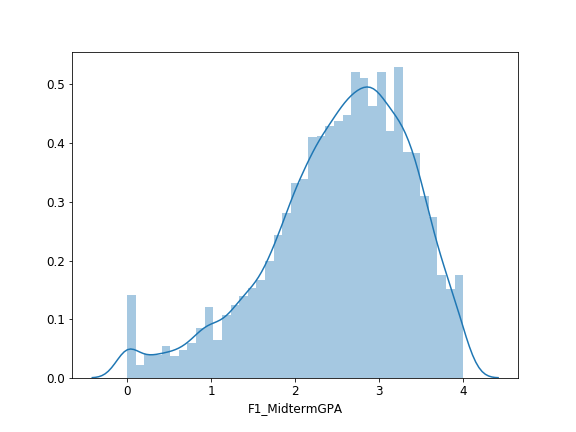
\includegraphics[scale=0.7]{F1-MidTermGPA-distribution}
	\caption{Distribution plot of the F1\_MidtermGPA}
	\label{fig:F1_MidtermGPA_plot}
\end{figure}

The F1\_MidtermGPA variable had 286 missing values which adds up to a very small percentage in the overall data. We analyzed the distribution plot of F1\_MidtermGPA (figure \ref{fig:F1_MidtermGPA_plot}) and noticed that it also follows a gaussian distribution with mean value of 2.5272 and a standard deviation of 0.851. Considering the above information we imputed the missing value of the variable with its mean as it would not shift the centrality of the variable.

\subsubsection {Imputing F1\_MathGradePass}
F1\_MathGradePass is a categorical variable with values 'Y' or 'N', where a 'Y' represents if a student got a passing grade in math taken during his first fall term and 'N' if he got a failing grade. It had a total of 4989 missing values in the variable. Such a large number of missing values for this variable is attributed to the fact that a student who did not take any math course will not have a value in this variable. Hence the missing value was replaced with a 'N'.

\subsection {Data Transformations}
Now that we have a cleaned dataset, we need to apply transformations on the data before they can be inputted to a machine learning algorithm. This step is essential as our dataset has a lot of categorical variables which need to be converted to numerical values before we perform any further analysis. 

The general approach is to encode the categories with numerical values. One-hot encoding is a popular encoding technique used in machine learning in which a categorical variable is converted into a binary vector, where each possible value of the categorical variable is assigned to a dummy variable with a default value of '0' and the dummy variable which was the value of the categorical variable will have the value '1'. In simple terms, applying one-hot encoding to a categorical variable results in an one-hot vector, where only one element is non-zero, or hot. There were a total of 23 categorical variables in our raw dataset which were one-hot encoded to yield a total of 85 variables. We noticed that applying transformations on our raw data resulted in a huge increase in the number of variables available for analysis. Having more number of variables can result in poor performance of the model, as there might be some variables that are redundant and irrelevant to our prediction problem. To handle such scenarios, feature selection is useful as it automates the process of selecting features that are important to the prediction model. The next subsection describes in detail about the feature selection process used in this thesis.




\subsection {Feature Selection}
\begin{table}
	\renewcommand{\arraystretch}{1.3}
	\caption{Tests based on type of input and output variables}
	\label{table:statistical_db}
	\centering
	\begin{tabular}{|c|c|c|c|}
    \hline
    \multicolumn{2}{|c|}{} & \multicolumn{2}{|c|}{ \bfseries Response Type}\\ \cline{3-4}
      \multicolumn{2}{|c|}{} & \bfseries Quantitative & \bfseries Categorical\\ \hline
     \multirow{2}{*}{ \bfseries Feature type}   &  \bfseries Quantitive & Correlation & Chi-Square Test \\ \cline{2-4}
     & \bfseries Categorical & ANOVA & Chi-Square Test\\
    \hline

\end{tabular}
\end{table}
Feature selection is the process of identifying and selecting features from our raw data that contribute most to the prediction of our output variable. Feature selection methods are useful to identify and remove unneeded, irrelevant and redundant attributes from data that do not contribute to the accuracy of a predictive model. There are various feature selection methods available in machine learning that can be applied to the available dataset. One key factor to consider before using a particular method is to have an idea of the models you are going to use on your data. 

One of the feature selection approaches deals with the idea of identifying the relationship of features with the output variable to decide their importances. To find such relationships, we need to identify the data type of features and the output variable. The table \ref{table:statistical_db} shows the types of tests used based on input feature types and output response types. The tests are as follows: 

\noindent \textbf{Correlation} : In general, we use the Pearson correlation coefficient to measure the strength of a linear association between two numerical variables. The higher the magnitude of the correlation coefficient, the greater is the variables influence on predicting output variable.

\noindent \textbf{ANOVA} : ANOVA refers to "Analysis of Variance" which is a collection of statistical models and their associated procedures (such as "variation" among and between groups) used to analyze the differences among group means.

\noindent \textbf{Chi-Square} : A chi-square test, also written as $\tilde{\chi}^2$ test is used to determine whether there is a significant difference between the expected frequencies and the observed frequencies in one or more categories.

In our dataset, the response variable is a categorical with categories \{'Y' , 'N'\} and input features are both categorical and quantitative. Hence an appropriate choice of test to find relationships between the input features and output response is to use the Chi-square test. In machine learning the process of using such statistical tests on the dataset is known as Univariate selection. Hence univariate selection using Chi-Square test was applied on the transformed dataset to yield 51 important features as opposed to the 85 features obtained after data transformation.





\section{Exploratory Data Analysis}
Exploratory data analysis (EDA) is an approach employed to analyze data sets and summarize their main characteristics, often with visual methods, without making any assumptions about its contents. It is an important step to take before diving into statistical modeling or predictive analysis because it provides the important information and context needed to develop an appropriate model for the problem. In this section we try to uncover some important patterns inherent in our data with appropriate plots.

\begin{figure}
	\centering
	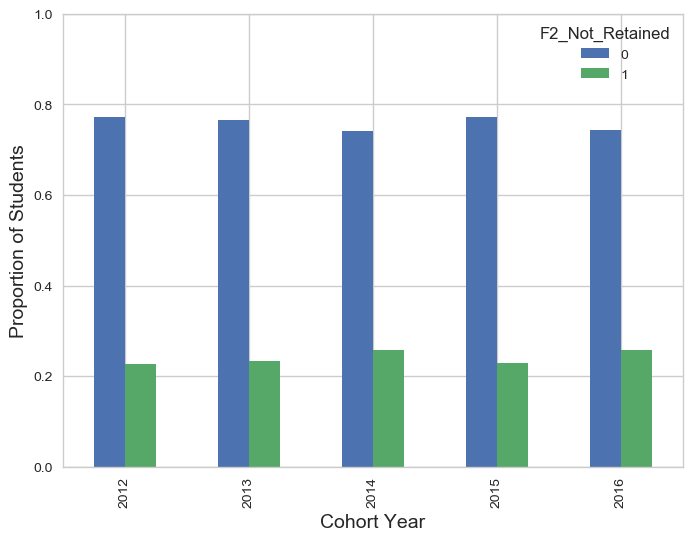
\includegraphics[scale=0.6]{NotRetained_fre_acadyear}
	\caption{Academic Year vs F2\_NotRetained}
	\label{fig:AcadYear_F2NotRetained_plot}
\end{figure}


\subsection {Academic year Vs F2\_Not\_Retained}

To understand the distribution of student dropouts at the end of each year, we plotted the proportions of the outcome variable F2\_Not\_Retained for each year as shown in Figure \ref{fig:AcadYear_F2NotRetained_plot}. Each academic year represents the cohort of students who were in their F1 semester in that specific year. From the plot, we can infer that the number of students who drop out after their first-year varies very slightly over the recent years. More importantly, we see a pattern of increasing student dropout rates as opposed to an expected decrease even though efforts are being made by educators at UNLV to improve the student retention rates.


\subsection {IPEDS\_Race Vs F2\_Not\_Retained}
In this section, we tried to analyze the patterns observed by different categories of the IPEDS Race with respect to student retention. For this, we first plotted the different IPEDS Race categories on x-axis and the count of students belonging to that particular race on y-axis as shown in figure \ref{fig:ipeds_F2NotRetained_plot}. We observed that the student population of different races was very different at UNLV with higher populations belonging to Asian, Hispanic and White races.


\begin{figure}[!ht]
	\centering
	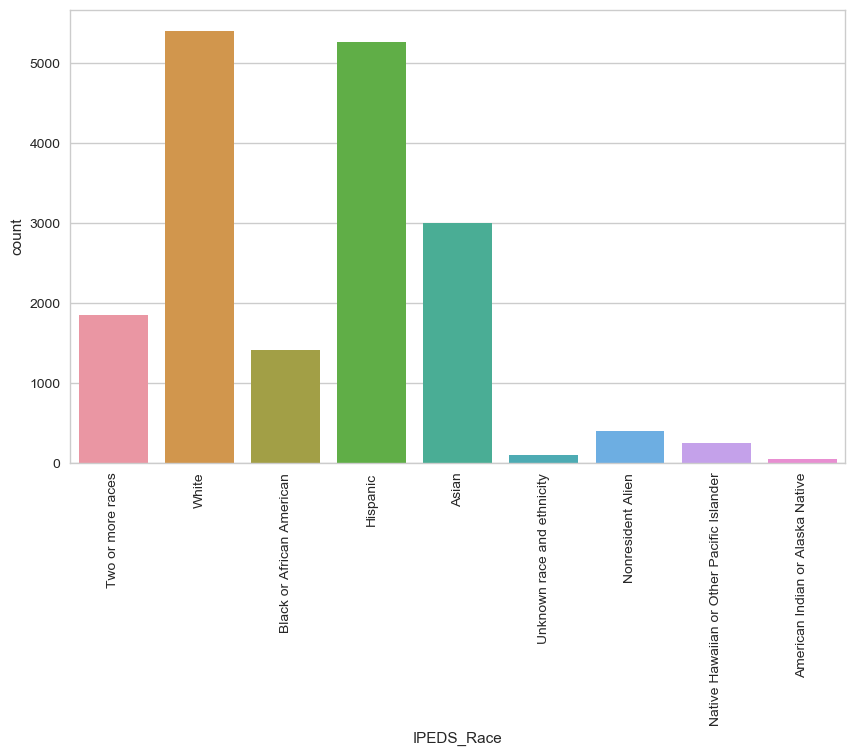
\includegraphics[scale=0.70]{NotRetained_ipeds}
	\caption{Count plot of IPEDS\_Race variable}
	\label{fig:ipeds_F2NotRetained_plot}
\end{figure}

Although fig \ref{fig:ipeds_F2NotRetained_plot} gives us a good idea about the type of students at UNLV, it is not sufficient to help us understand the retention patterns among the different categories. For this, we calculated the retention rates of each race category and tabulated them in table \ref{table:ipeds_race_retentions}. Considering the student distributions in each race category and their retention rates from table, we conclude that the Asian race category had the highest student retention followed by Hispanic and White categories. On the whole we observe that the student's race is useful in predicting if he/she will be retained after the first year.

 \begin{table}[!t]
	\renewcommand{\arraystretch}{1.3}
	\caption{Retention Rates of each IPEDS Race Category}
	\label{table:ipeds_race_retentions}
	\centering
	\begin{tabular}{|c|c|c|}
		\hline
		\bfseries IPEDS Race & \bfseries F2\_Retained & \bfseries F2\_Not\_Retained\\
		\hline
		Asian & 85.75\% & 14.25\% \\ \hline
		American Indian or Alaska Native & 53.48\% & 46.51\% \\ \hline
		Black or African American & 66.83\% & 33.17\% \\ \hline
		Hispanic & 74.34\% & 25.66\% \\ \hline
		Native Hawaiian or Other Pacific Islander & 68.65\% & 31.35\% \\ \hline
		Nonresident Alien & 86.14\% & 13.86\% \\ \hline
		Two or more races &  74.23\% &  25.76\% \\ \hline
		Unknown race and ethnicity & 75.26 \% & 24.74\% \\ \hline
		White & 74.38\% & 25.61\% \\ \hline
	\end{tabular}
\end{table}



\subsection {Mom\_Edu\_Level	 Vs F2\_Not\_Retained}
The variable Mom\_Edu\_Level represents the highest education level of a student's mother. In this section, we tried to analyze the patterns observed by different categories of this variable with respect to student retention. For this, we plotted the different categories of Mom\_Edu\_Level variable on x-axis and the count of students whose Mom's education level belonged to that category on y-axis as shown in figure \ref{fig:mom_edu_F2NotRetained_plot}. We observed that the education level of the Mom's of students at UNLV was highly distributed. It especially gives us the information that most of the student's Mom's had a minimum education of High School or more. However this does not explain much about the effect of Mom's education level on student's retention.

\begin{figure}[!ht]
	\centering
	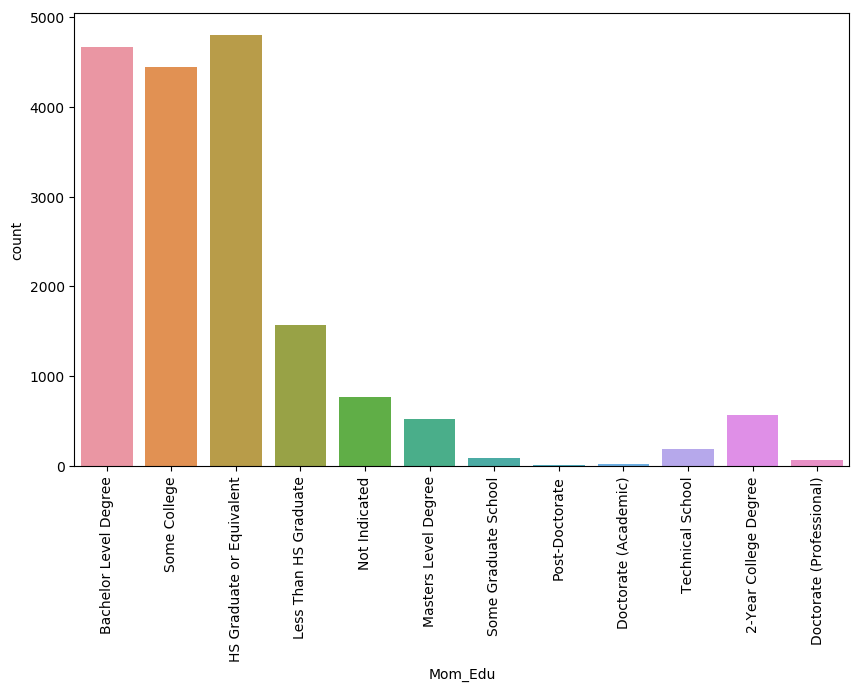
\includegraphics[scale=0.65]{mom_edu_countplot}
	\caption{Count plot of Mom\_Edu\_Level variable}
	\label{fig:mom_edu_F2NotRetained_plot}
\end{figure}

\begin{table}[!t]
	\renewcommand{\arraystretch}{1.3}
	\caption{Retention Rates of different categories of Mom\_Edu\_Level variable}
	\label{table:mom_edu_retentions}
	\centering
	\begin{tabular}{|c|c|c|}
		\hline
		\bfseries Mom's Education Level & \bfseries F2\_Retained & \bfseries F2\_Not\_Retained\\
		\hline
		Post-Doctorate  & 100.00\%  & 00.00\% \\ \hline
		Doctorate (Professional) & 84.37\% &  15.62\% \\ \hline
		Doctorate (Academic) & 77.78\% & 22.22\% \\ \hline
		Masters Level Degree    &   76.14\% &  23.86\% \\ \hline
		Bachelor Level Degree &  78.76\%  & 21.24\% \\ \hline
		Some College & 74.76\% & 25.24\% \\ \hline
		Some Graduate School  & 78.82\% &  21.17\% \\ \hline
		2-Year College Degree    &  74.82\%  & 25.18\% \\ \hline
		HS Graduate or Equivalent  & 74.20\% &  25.79\% \\ \hline
		Less Than HS Graduate     & 74.52\% &  25.47\% \\ \hline
		Technical School  &         69.64\% &  30.36\% \\ \hline
		Not Indicated         &    77.46\% & 22.53\% \\ \hline
	\end{tabular}
\end{table}



To get a better understanding of the effect of Mom's Education on students retention, we calculated the retention rates of students from each category of the variable and tabulated them in table \ref{table:mom_edu_retentions}. Considering the student distributions in each category and the retention rates of the variable from table, we notice some expected patterns such as more students were retained if their Mom had an Education level higher than bachelor's. But strangely we also noticed that the retention rate of students with their Mom's education level as Less than HS Graduate was also good at UNLV. This gives us a hint of the variability of patterns inherent in the students data from UNLV.


\subsection {Dad\_Edu\_Level Vs F2\_Not\_Retained}
The variable Dad\_Edu\_Level represents the highest education level of a student's father. In this section, we tried to analyze the patterns observed by different categories of the Dad\_Edu\_Level variable with respect to student retention. For this, we plotted the different categories of Dad\_Education\_Level variable on x-axis and the count of students belonging to that category on y-axis as shown in figure \ref{fig:dad_edu_F2NotRetained_plot}. We observed that the education level of the Dad's of students at UNLV was highly distributed. It especially gives us the information that most of the student's Dad's had a minimum education of High School or more.

\begin{figure}
	\centering
	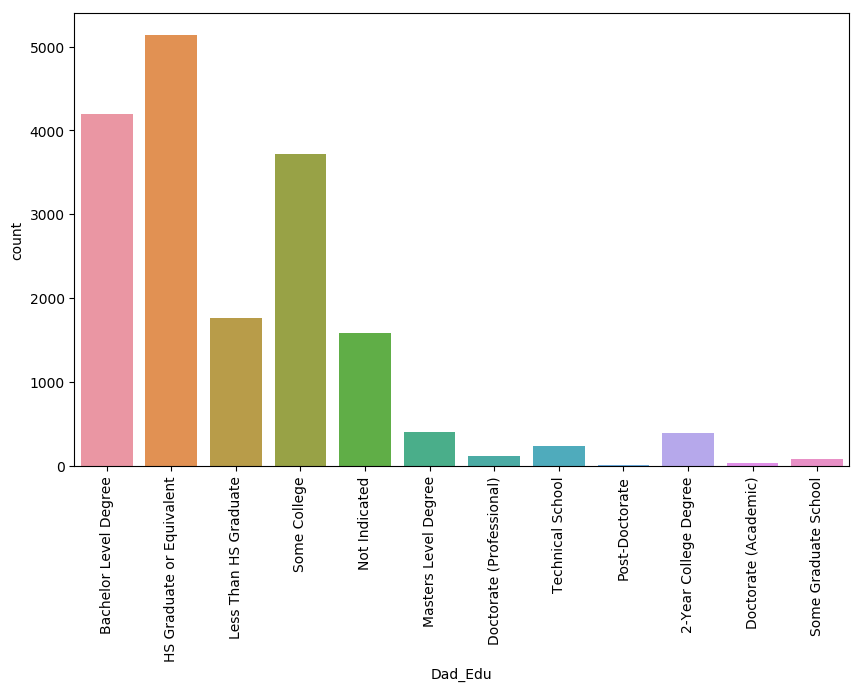
\includegraphics[scale=0.65]{dad_edu_countplot}
	\caption{Count plot of Dad\_Edu\_Level variable }
	\label{fig:dad_edu_F2NotRetained_plot}
\end{figure}

\begin{table}
	\renewcommand{\arraystretch}{1.3}
	\caption{Retention Rates of different categories of Dad\_Edu\_Level variable}
	\label{table:dad_edu_retentions}
	\centering
	\begin{tabular}{|c|c|c|}
		\hline
		\bfseries Dad's Education Level & \bfseries F2\_Retained & \bfseries F2\_Not\_Retained\\
		\hline
		Post-Doctorate  & 86.66\%  & 13.34\% \\ \hline
		Doctorate (Professional) & 77.86\% &  22.14\% \\ \hline
		Doctorate (Academic) & 86.84\% & 13.16\% \\ \hline
		Masters Level Degree    &   75.80\% &  24.20\% \\ \hline
		Bachelor Level Degree &  80.34\%  & 19.66\% \\ \hline
		Some College & 76.30\% & 23.70\% \\ \hline
		Some Graduate School  & 76.62\% &  23.38\% \\ \hline
		2-Year College Degree    &  81.15\%  & 19.75\% \\ \hline
		HS Graduate or Equivalent  & 73.36\% &  26.64\% \\ \hline
		Less Than HS Graduate     & 73.86\% &  26.14\% \\ \hline
		Technical School  &         69.50\% &  30.50\% \\ \hline
		Not Indicated         &    71.78\% & 28.22\% \\ \hline
	\end{tabular}
\end{table}

To get a better understanding of the effect of Dad's Education on students retention, we calculated the retention rates of students from each category of the variable and tabulated them in table  \ref{table:dad_edu_retentions}. Considering the student distributions in each category and the retention rates of the variable from table, we notice many expected patterns such as more students were retained if their Dad had an Education level higher than bachelors'. But strangely, we also noticed that the retention rate of students with their Dad's education level as Less than HS Graduate was also good at UNLV. This gives us a hint of the variability of patterns inherent in the students data from UNLV.


\begin{figure}
	\centering
	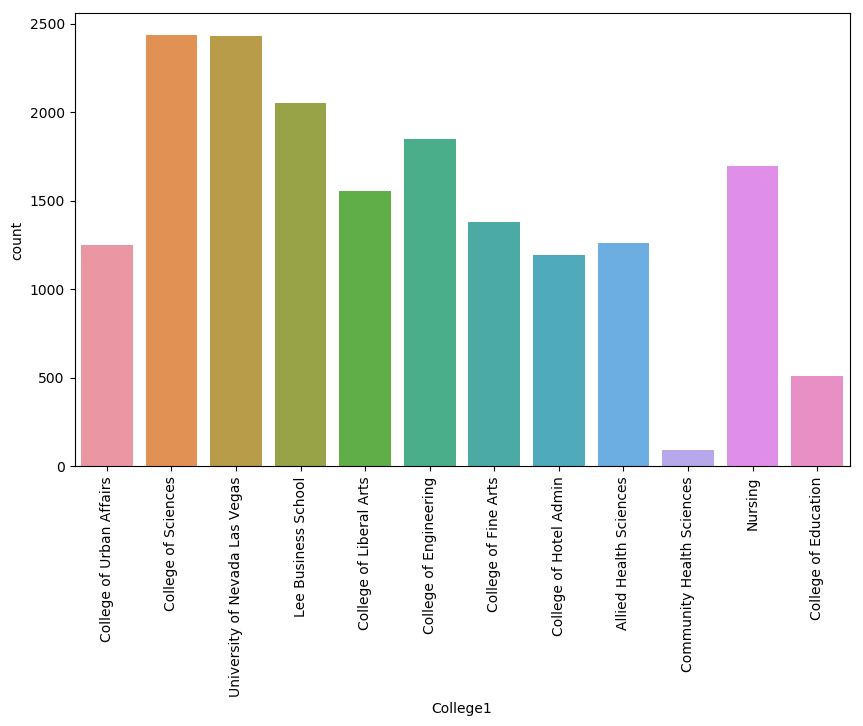
\includegraphics[scale=0.65]{college_countplot}
	\caption{Count plot of College1 variable}
	\label{fig:college_F2NotRetained_plot}
\end{figure}

\subsection {College1 Vs F2\_Not\_Retained}
The variable College1 represents the name of the college of the student during his first year. In this section, we tried to analyze the patterns observed by different categories of the student's college in his F1 term with respect to student retention. For this, we plotted the different categories of College1 variable on x-axis and the count of students belonging to that category on y-axis as shown in figure \ref{fig:college_F2NotRetained_plot}. We observed that the count of students belonging to a college was quite distributed with more students from College of Sciences followed by Lee Business school.


\begin{table}
	\renewcommand{\arraystretch}{1.3}
	\caption{Retention Rates of different categories of College1 variable}
	\label{table:college_retentions}
	\centering
	\begin{tabular}{|l|c|c|}
		\hline
		\bfseries College1 & \bfseries F2\_Retained & \bfseries F2\_Not\_Retained\\
		\hline
		College of Hotel Admin  & 80.98\%  & 19.02\% \\ \hline
		College of Sciences & 78.62\% &  21.38\% \\ \hline
		College of Engineering & 77.63\% & 23.37\% \\ \hline
		College of Education    &   77.73\% &  23.27\% \\ \hline
		College of Fine Arts &  76.61\%  & 23.39\% \\ \hline
		College of Liberal Arts & 76.06\% & 23.94\% \\ \hline
		Lee Business School  & 75.31\% &  24.69\% \\ \hline
		Nursing    &  75.14\%  & 24.86\% \\ \hline
		Allied Health Sciences  & 73.53\% &  26.57\% \\ \hline
		University of Nevada Las Vegas     & 73.07\% &  26.93\% \\ \hline
		College of Urban Affairs  &         70.97\% &  29.03\% \\ \hline
		Community Health Sciences         &    64.51\% & 35.59\% \\ \hline
	\end{tabular}
\end{table}


To get a better understanding of the effect of student's college on retention, we calculated the retention rates of each college and tabulated them in table \ref{table:college_retentions}. Considering the student distributions in each college and the retention rates of the colleges from the table \ref{table:college_retentions}, we notice few patterns such as more students were retained in College of Sciences and College of Engineering which had higher student counts. Even though other colleges had lesser student populations, their student retention rates were similar and averaged to about 75\% . This gives us a hint of the variability of patterns inherent in the students data from UNLV.


\chapter{Building Models} \label{chapter:building_models}

\section {Data Splitting }

Once the dataset was cleaned and feature selection was performed on it, there were 51 variables excluding the F2\_Not\_Retained variable. Hence, we have a total of 51 independent variables which act as predictors and are inputted into the model to predict the value of F2\_Not\_Retained the output variable. 

The data was split based on the academic year, so it will be easy to analyze and test the retention rates on individual students as well as the whole academic year. The count of students in each academic year is shown in Table \ref{table:acad_db}.

\begin{table}[!htbp]
	\renewcommand{\arraystretch}{1.3}
	\caption{Count of students in each academic year}
	\label{table:acad_db}
	\centering
	\begin{tabular}{|c|c|}
    \hline
    \bfseries Academic Year & \bfseries Count of Students \\ 
    \hline
  	2012 &  2996 \\ \hline
	2013 & 3585 \\ \hline
	2014 & 3656 \\ \hline
	2015 & 3715 \\ \hline
	2016 & 3756 \\ \hline
\end{tabular} 
\end{table}

From the entire dataset, the student records from the academic years 2012, 2013 ,2014 and 2015 were combined to form the train\_test dataset. The remaining student records from the year 2016 were used to form test\_unseen dataset. The idea was to use the 4 years of data to train, test and evaluate the model. Once the model is trained and tested, it will be used to make predictions on student records from the test\_unseen dataset. This way, by not using any data from the 2016 academic year in training and testing processes, the model will treat it as totally unseen data and makes predictions which will not be based on any assumptions on the data of that year. There were a total of 13,192 student records in the train\_test dataset and 3756 student records in test\_unseen dataset.

Seventy percent (70\%) of the train\_test dataset were used to train the selected models. The remaining thirty percent (30\%) was used to test, evaluate and compare the performances of the trained models. 

\section {Experiments on Models}
Once the training, testing and unseen data were created from the original dataset, each of the selected models were trained using the training data and evaluated on the test data. The models which were trained were Logistic Regression, Decision Tree, Random Forest and Support Vector Machines. 

Once each model was trained, we used it to make predictions and generate a confusion matrix on the test data. The confusion matrix was used to calculate the classification accuracy, sensitivity, specificity, precision, F\textsubscript{1} scores and plot the ROC curve for the model. We also applied K-fold cross-validation on the training data to get the cross-validated AUC value, that was used to verify if the model results were not biased. If the cross-validated AUC score was similar to the one we get from the predictions on test data, it means that the model is actually learning from the training data. Furthermore, we use the trained model to make predictions on unseen data and generate confusion matrix to compute the performance metrics which give us a better idea of the generalizing power of the model on unseen data.

All the above-mentioned performance metrics were used to compare the models to find the one that suits best for the UNLV students data. 

\subsection {Logistic Regression}
A Logistic Regression (LR) model was created using the sklearn package in python and it was fitted on the training data. The trained model was then used to perform predictions on the test data. The confusion matrix generated from the predictions of the test data is as shown in Figure \ref{fig:lr_confusion_matrix}

  \begin{figure}
	\centering
	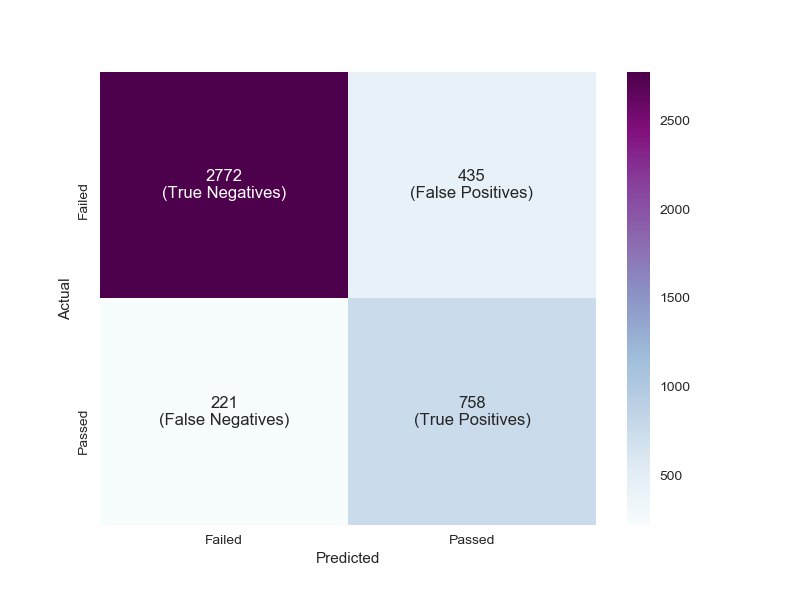
\includegraphics[scale=0.6]{LR-Confusion_matrix}
	\caption{Confusion Matrix of Logistic Regression on test data}
	\label{fig:lr_confusion_matrix}
\end{figure} 

The logistic regression model built on the training data had a classification accuracy of 0.843. The table \ref{table:lr-metrics_db} shows the other metrics calculated from the confusion matrix in Figure \ref{fig:lr_confusion_matrix}. 
\begin{table}
	\renewcommand{\arraystretch}{1.3}
	\caption{Computed metrics based on actual and predicted test data values using LR model}
	\label{table:lr-metrics_db}
	\centering
	\begin{tabular}{|c|c|c|c|c|c|c|}
    \hline
  	 & \bfseries Accuracy & \bfseries Sensitivity & \bfseries Specificity & \bfseries Precision & \bfseries F\textsubscript{1} Score  & \bfseries AUC\\  
    \hline
	LR model & 0.843 & 0.774 & 0.864 & 0.635 & 0.70 & 0.882 \\ \hline
	\end{tabular} 
\end{table}


 \begin{figure}[!htb]
	\centering
	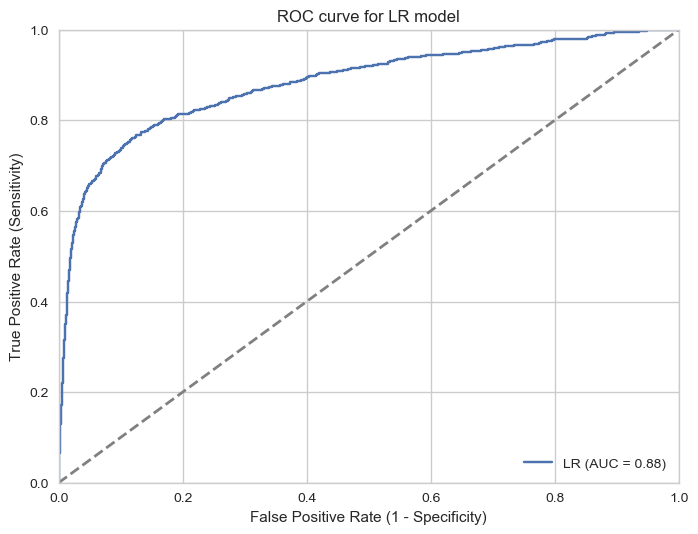
\includegraphics[scale=0.6]{LR-roc}
	\caption{ROC curve for Logistic Regression on test data}
	\label{fig:lr_roc}
\end{figure} 

ROC curve for the LR model on test data was plotted and is as shown in the figure \ref{fig:lr_roc} . K-Fold cross validation with the k value of 10 was applied on the training data to get a cross validated AUC score of 0.88. This clearly confirms that the model is actually learning from the training data and is in fact generalizing the unseen data well.

The trained LR model was used to perform predictions on the unseen dataset that was created from the original dataset. The predictions on the unseen data define the generalizing power of the LR model at the individual student level as well as the academic year level. The confusion matrix generated from the predictions on unseen data is as shown in figure \ref{fig:lr_unseen_confusion_matrix}.

  \begin{figure}[!htb]
	\centering
	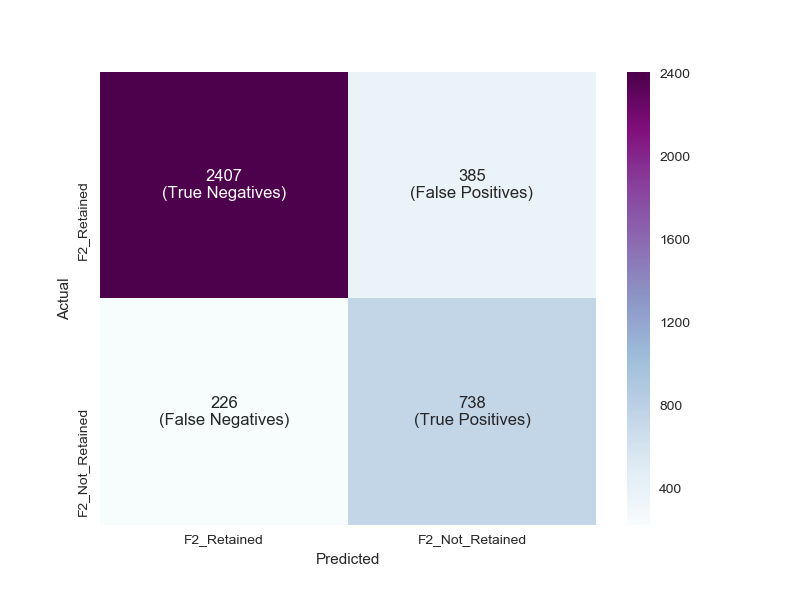
\includegraphics[scale=0.6]{LR-unseen-Confusion_matrix}
	\caption{Confusion Matrix of Logistic Regression on unseen data viz 2016 academic year data}
	\label{fig:lr_unseen_confusion_matrix}
\end{figure} 


The logistic regression model built on the training data had a classification accuracy of 0.843 on the unseen data. The table \ref{table:lr-unseen_metrics_db} shows the other metrics calculated from the confusion matrix in Figure \ref{fig:lr_unseen_confusion_matrix}.

\begin{table}[!htb]
	\renewcommand{\arraystretch}{1.3}
	\caption{Computed metrics based on actual and predicted unseen data values using LR model}
	\label{table:lr-unseen_metrics_db}
	\centering
	\begin{tabular}{|c|c|c|c|c|c|c|}
    \hline
  	 & \bfseries Accuracy & \bfseries Sensitivity & \bfseries Specificity & \bfseries Precision & \bfseries F\textsubscript{1} Score  & \bfseries AUC\\  
    \hline
	LR model & 0.837 & 0.766 & 0.862 & 0.657 & 0.71 & 0.883 \\ \hline
	\end{tabular} 
\end{table}

\subsection {Decision Trees}
A Decision tree (DTree) model was created using the sklearn package in python and it was fitted on the training data. The trained model was then used to perform predictions on the test data. The confusion matrix generated from the predictions of the test data is as shown in Figure \ref{fig:Dtree_confusion_matrix}

  \begin{figure}[!htb]
	\centering
	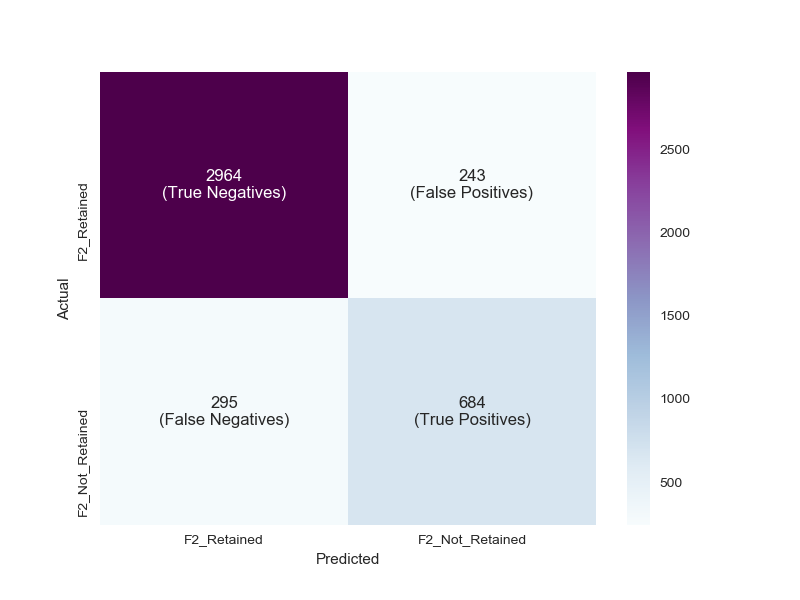
\includegraphics[scale=0.6]{DTree-Confusion_matrix}
	\caption{Confusion Matrix of Decision Tree on test data}
	\label{fig:Dtree_confusion_matrix}
\end{figure} 

The decision tree model built on the training data had a classification accuracy of 0.871. The table \ref{table:Dtree_confusion_matrix} shows the other metrics calculated from the confusion matrix in Figure \ref{fig:Dtree_confusion_matrix}. 
\begin{table} [!htb]
	\renewcommand{\arraystretch}{1.3}
	\caption{Computed metrics based on actual and predicted test data values using DTree model}
	\label{table:Dtree_confusion_matrix}
	\centering
	\begin{tabular}{|c|c|c|c|c|c|c|}
    \hline
  	 & \bfseries Accuracy & \bfseries Sensitivity & \bfseries Specificity & \bfseries Precision & \bfseries F\textsubscript{1} Score  & \bfseries AUC\\  
    \hline
	DTree model & 0.871 & 0.699 & 0.924 & 0738 & 0.72 & 0.860 \\ \hline
	\end{tabular} 
\end{table}

 \begin{figure}[!htbp]
	\centering
	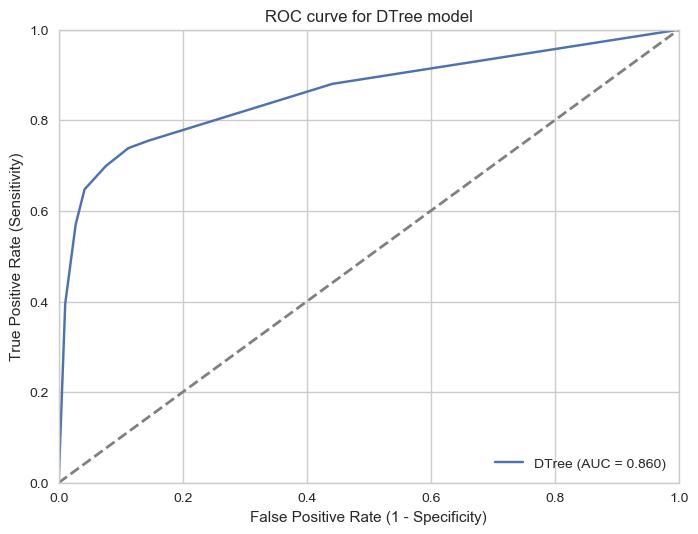
\includegraphics[scale=0.6]{DTree-roc}
	\caption{ROC curve for Decision Tree on test data}
	\label{fig:DTree_roc}
\end{figure} 

ROC curve for the DTree model on test data was plotted and is as shown in the figure \ref{fig:DTree_roc} . K-Fold cross validation with the k value of 10 was applied on the training data to get a cross validated AUC score of 0.86. This clearly confirms that the model is actually learning from the training data and is in fact generalizing the unseen data well.

The trained DTree model was used to perform predictions on the unseen dataset that was created from the original dataset. The predictions on the unseen data define the generalizing power of the Dtree model at the individual student level as well as the academic year level. The confusion matrix generated from the predictions on unseen data is shown in the figure \ref{fig:DTree_unseen_confusion_matrix}.

  \begin{figure}[!htb]
	\centering
	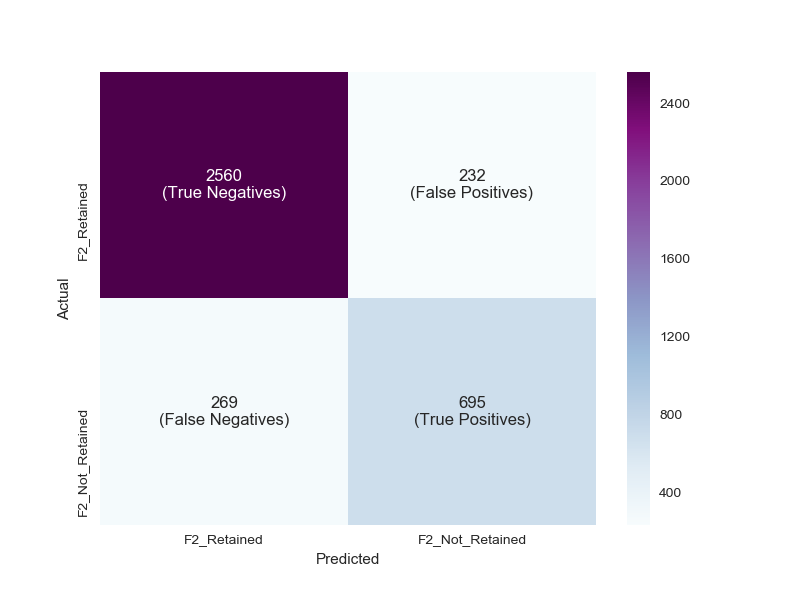
\includegraphics[scale=0.6]{DTree-unseen-Confusion_matrix}
	\caption{Confusion Matrix of Decision Tree on unseen data viz 2016 academic year data}
	\label{fig:DTree_unseen_confusion_matrix}
\end{figure} 


The decision tree model built on the training data had a classification accuracy of 0.867 on the unseen data. The Table \ref{table:DTree-unseen_metrics_db} shows the other metrics calculated from the confusion matrix in Figure \ref{fig:DTree_unseen_confusion_matrix}.

\begin{table}[!htb]
	\renewcommand{\arraystretch}{1.3}
	\caption{Computed metrics based on actual and predicted unseen data values using DTree model}
	\label{table:DTree-unseen_metrics_db}
	\centering
	\begin{tabular}{|c|c|c|c|c|c|c|}
    \hline
  	 & \bfseries Accuracy & \bfseries Sensitivity & \bfseries Specificity & \bfseries Precision & \bfseries F\textsubscript{1} Score  & \bfseries AUC\\  
    \hline
	DTree model & 0.867 & 0.721 & 0.917 & 0.750 & 0.74 & 0.87 \\ \hline
	\end{tabular} 
\end{table}


\subsection {Random Forest}
A Random Forest (RF) model was created using the sklearn package in python and it was fitted on the training data. The trained model was then used to perform predictions on the test data. The confusion matrix generated from the predictions of the test data is as shown in the Figure \ref{fig:RF_confusion_matrix}

  \begin{figure}[!htb]
	\centering
	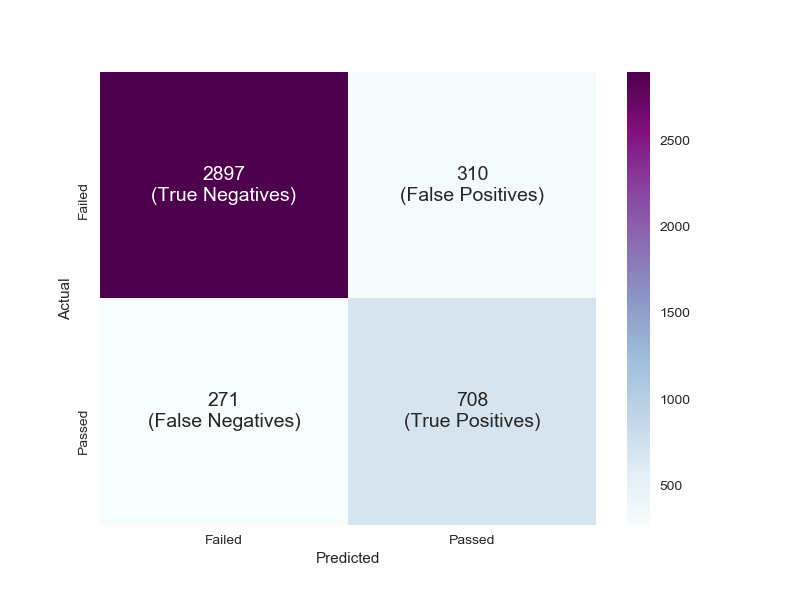
\includegraphics[scale=0.6]{RF-Confusion_matrix}
	\caption{Confusion Matrix of Random Forest on test data}
	\label{fig:RF_confusion_matrix}
\end{figure} 

The Random Forest model built on the training data had a classification accuracy of 0.861. The Table \ref{table:RF_confusion_matrix} shows the other metrics calculated from the confusion matrix in Figure \ref{fig:RF_confusion_matrix}. 
\begin{table}
	\renewcommand{\arraystretch}{1.3}
	\caption{Computed metrics based on actual and predicted test data values using RF model}
	\label{table:RF_confusion_matrix}
	\centering
	\begin{tabular}{|c|c|c|c|c|c|c|}
    \hline
  	 & \bfseries Accuracy & \bfseries Sensitivity & \bfseries Specificity & \bfseries Precision & \bfseries F\textsubscript{1} Score  & \bfseries AUC\\  
    \hline
	RF model & 0.861 & 0.723 & 0.903 & 695 & 0.71 & 0.876 \\ \hline
	\end{tabular} 
\end{table}

 \begin{figure}[!htb]
	\centering
	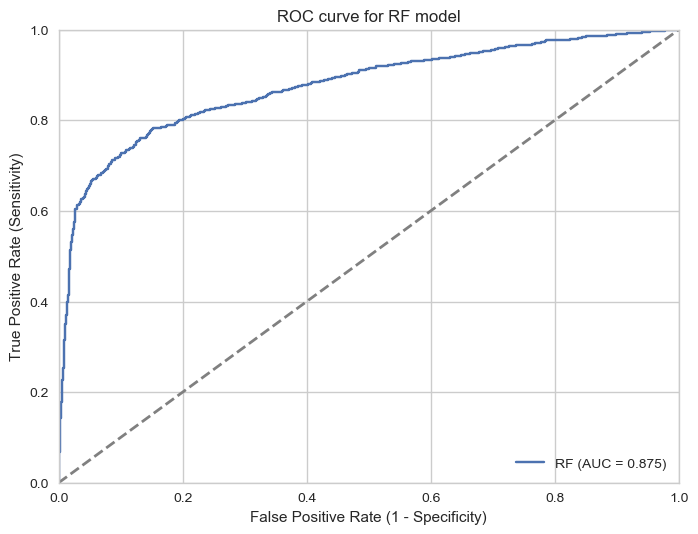
\includegraphics[scale=0.6]{RF-roc}
	\caption{ROC curve for Random Forest on test data}
	\label{fig:RF_roc}
\end{figure} 

ROC curve for the RF model on test data was plotted and is as shown in the figure \ref{fig:RF_roc} . K-Fold cross validation with the k value of 10 was applied on the training data to get a cross validated AUC score of 0.876. This clearly confirms that the model is actually learning from the training data and is in fact generalizing the unseen data well.

The trained RF model was used to perform predictions on the unseen dataset that was created from the original dataset. The predictions on the unseen data define the generalizing power of the RF model at the individual student level as well as the academic year level.. The confusion matrix generated from the predictions on unseen data is shown in the figure \ref{fig:RF_unseen_confusion_matrix}.

  \begin{figure}[!htb]
	\centering
	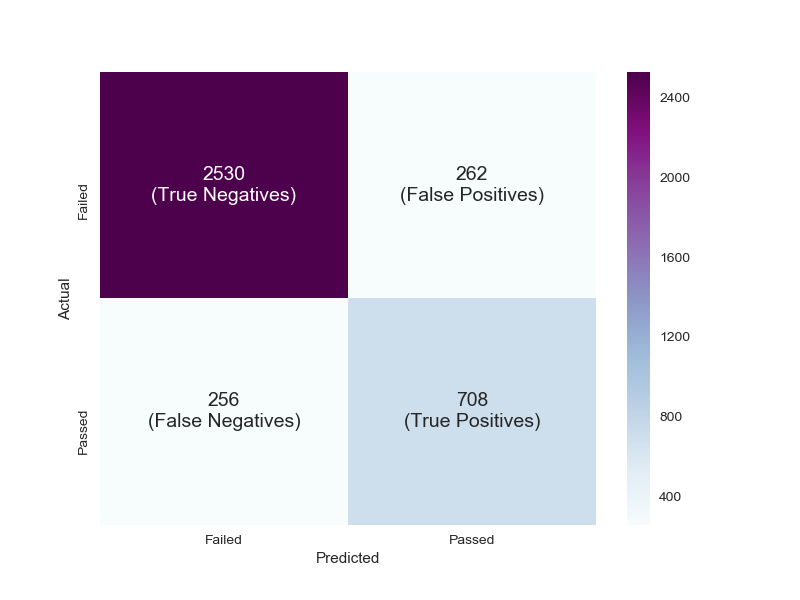
\includegraphics[scale=0.6]{RF-unseen-Confusion_matrix}
	\caption{Confusion Matrix of Random Forest on unseen data viz 2016 academic year data}
	\label{fig:RF_unseen_confusion_matrix}
\end{figure} 


The decision tree model built on the training data had a classification accuracy of 0.867 on the unseen data. The Table \ref{table:RF-unseen_metrics_db} shows the other metrics calculated from the confusion matrix in Figure \ref{fig:RF_unseen_confusion_matrix}.

\begin{table}[!htb]
	\renewcommand{\arraystretch}{1.3}
	\caption{Computed metrics based on actual and predicted unseen data values using RF model}
	\label{table:RF-unseen_metrics_db}
	\centering
	\begin{tabular}{|c|c|c|c|c|c|c|}
    \hline
  	 & \bfseries Accuracy & \bfseries Sensitivity & \bfseries Specificity & \bfseries Precision & \bfseries F\textsubscript{1} Score  & \bfseries AUC\\  
    \hline
	RF model & 0.867 & 0.721 & 0.917 & 0.750 & 0.74 & 0.87 \\ \hline
	\end{tabular} 
\end{table}


\subsection {Support Vector Machines}
A Support Vector Machine (SVM) model was created using the sklearn package in python and it was fitted on the training data. The trained model was then used to perform predictions on the test data. The confusion matrix generated from the predictions of the test data is as shown in Figure \ref{fig:SVM_confusion_matrix}

  \begin{figure}[!htb]
	\centering
	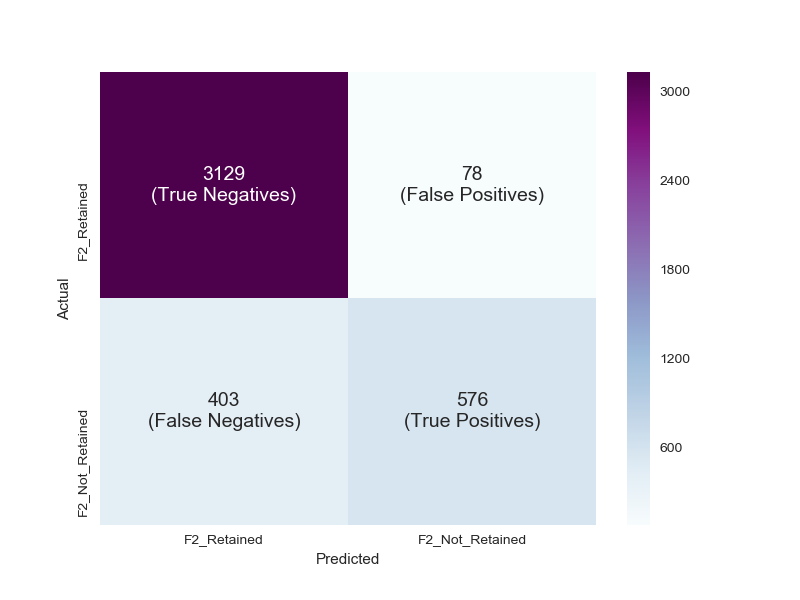
\includegraphics[scale=0.6]{SVM-Confusion_matrix}
	\caption{Confusion Matrix of Support Vector Machine model on test data}
	\label{fig:SVM_confusion_matrix}
\end{figure} 

The decision tree model built on the training data had a classification accuracy of 0.885. The table \ref{table:SVM_confusion_matrix} shows the other metrics calculated from the confusion matrix in Figure \ref{fig:SVM_confusion_matrix}. 
\begin{table} [!htb]
	\renewcommand{\arraystretch}{1.3}
	\caption{Computed metrics based on actual and predicted test data values using SVM model}
	\label{table:SVM_confusion_matrix}
	\centering
	\begin{tabular}{|c|c|c|c|c|c|c|}
    \hline
  	 & \bfseries Accuracy & \bfseries Sensitivity & \bfseries Specificity & \bfseries Precision & \bfseries F\textsubscript{1} Score  & \bfseries AUC\\  
    \hline
	SVM model & 0.885 & 0.588 & 0.976 & 881 & 0.71 & 0.857 \\ \hline
	\end{tabular} 
\end{table}

 \begin{figure}[!htb]
	\centering
	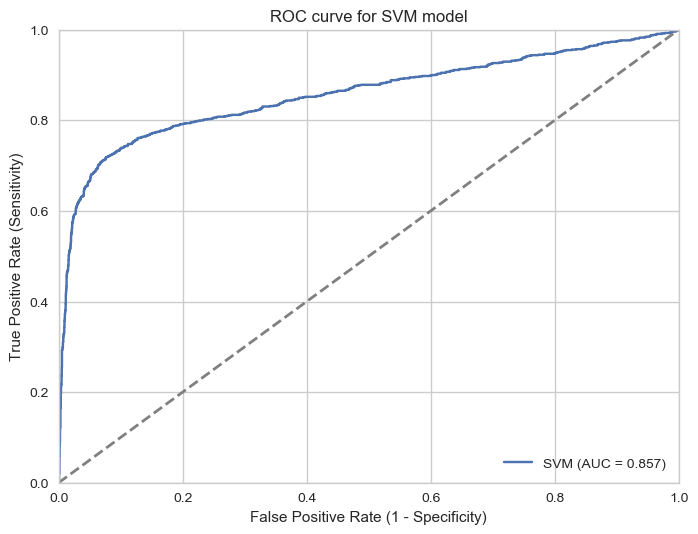
\includegraphics[scale=0.6]{SVM-roc}
	\caption{ROC curve for Decision Tree on test data}
	\label{fig:SVM_roc}
\end{figure} 

ROC curve for the SVM model on test data was plotted and is as shown in the figure \ref{fig:SVM_roc} . K-Fold cross validation with the k value of 10 was applied on the training data to get a cross validated AUC score of 0.86. This clearly confirms that the model is actually learning from the training data and is in fact generalizing the unseen data well.

The trained SVM model was used to perform predictions on the unseen dataset that was created from the original dataset. The predictions on the unseen data define the generalizing power of the SVM model at the individual student level as well as the academic year level. The confusion matrix generated from the predictions on unseen data is shown in the figure \ref{fig:SVM_unseen_confusion_matrix}.

  \begin{figure}[!htb]
	\centering
	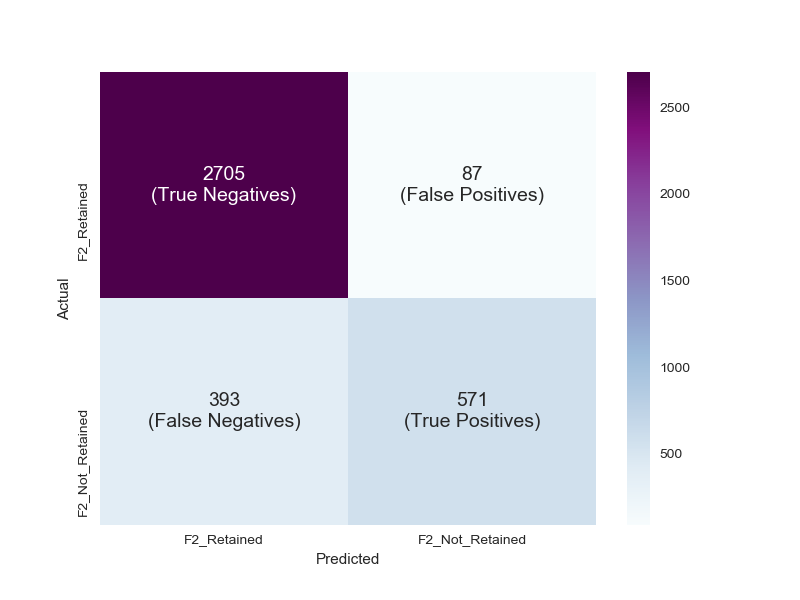
\includegraphics[scale=0.6]{SVM-unseen-Confusion_matrix}
	\caption{Confusion Matrix of SVM model on unseen data viz 2016 academic year data}
	\label{fig:SVM_unseen_confusion_matrix}
\end{figure} 


The support vector machine model built on the training data had a classification accuracy of 0.872 on the unseen data. The Table \ref{table:SVM-unseen_metrics_db} shows the other metrics calculated from the confusion matrix in Figure \ref{fig:SVM_unseen_confusion_matrix}.

\begin{table}[!htb]
	\renewcommand{\arraystretch}{1.3}
	\caption{Computed metrics based on actual and predicted unseen data values using SVM model}
	\label{table:SVM-unseen_metrics_db}
	\centering
	\begin{tabular}{|c|c|c|c|c|c|c|}
    \hline
  	 & \bfseries Accuracy & \bfseries Sensitivity & \bfseries Specificity & \bfseries Precision & \bfseries F\textsubscript{1} Score  & \bfseries AUC\\  
    \hline
	SVM model & 0.872 & 0.592 & 0.969 & 0.868 & 0.70 & 0.860 \\ \hline
	\end{tabular} 
\end{table}


\subsection {Comparison of the models}

\begin{table}
	\renewcommand{\arraystretch}{1.3}
	\caption{Comparison of metrics from different models on the training data}
	\label{table:compare_models_db}
	\centering
	\begin{tabular}{|c|c|c|c|c|c|c|}
    \hline
  	 & \bfseries Accuracy & \bfseries Sensitivity & \bfseries Specificity & \bfseries Precision & \bfseries F\textsubscript{1} Score  & \bfseries AUC\\  
    \hline
    	LR model & 0.843 & 0.774 & 0.864 & 0.635 & 0.70 & 0.882 \\ \hline
	DTree model & 0.871 & 0.699 & 0.924 & 0738 & 0.72 & 0.860 \\ \hline
	RF model & 0.861 & 0.723 & 0.903 & 695 & 0.71 & 0.876 \\ \hline
	SVM model & 0.885 & 0.588 & 0.976 & 881 & 0.71 & 0.857 \\ \hline
	\end{tabular} 
\end{table}


\subsection{Feature importance calculation based on selected models.} 
\subsection{Probability estimates to risk scores}
\chapter{Conclusion} \label{chapter:conclusion}

\subsection{Future Work}
%%%
%%% The bibliography - you can change the alpha to suit your style if you don't like it is it is.
%%% The bib file should be called 'thesis.bib' - if not then change the second line here to be correct.
\bibliographystyle{alpha}
\thesisbibliography{thesis}


%%%
%%% Vita comes next
\vita
\chapter{} %% please leave this one blank - the vita stuff is sort of a hack.
\linespread{1.3} 
\begin{center}
Graduate College\\
University of Nevada, Las Vegas\\[1cm]
Aditya Rajuladevi\\[1cm]
\end{center}

\noindent Degrees:\\
\indent Bachelor Degree in Computer Engineering 2014\\
\indent Jawaharlal Nehru Technological University, Hyderabad, India\\

\noindent Thesis Title: A Machine Learning Approach to Predict First-Year Student Retention Rates at University of Nevada, Las Vegas\\

\noindent Thesis Examination Committee:\\
\indent Chairperson, Dr. Fatma Nasoz, Ph.D.\\
\indent Committee Member, Dr. Laxmi Gewali, Ph.D.\\
\indent Committee Member, Dr. Justin Zhan, Ph.D.\\
\indent Graduate Faculty Representative, Dr. Magdalena Martinez, Ph.D.\\

\end{document}





